\documentclass[12pt]{article}
\usepackage{times}
\usepackage{geometry}
\geometry{letterpaper, portrait, margin=1in}
\usepackage[utf8]{inputenc}
\usepackage{enumitem,amssymb}
\usepackage{ragged2e}
\usepackage{natbib}
\usepackage{graphicx}
\newlist{thematic}{itemize}{8}
\setlist[thematic]{label=$\square$}
\usepackage{pifont}
\newcommand{\cmark}{\ding{51}}%
\newcommand{\xmark}{\ding{55}}%
\newcommand{\done}{\rlap{$\square$}{\raisebox{2pt}{\large\hspace{1pt}\cmark}}%
\hspace{-2.5pt}}
\newcommand{\wontfix}{\rlap{$\square$}{\large\hspace{1pt}\xmark}}
\usepackage{amsmath}    % Advanced maths commands
\usepackage{amssymb}    % Extra maths symbols


\def\aj{\rm AJ}
\def\araa{\rm ARA\&A}
\def\apj{\rm ApJ}
\def\apjl{\rm ApJ}
\def\apjs{\rm ApJS}
\def\ao{\rm Appl.~Opt.}
\def\apss{\rm Ap\&SS}
\def\aap{\rm A\&A}
\def\aapr{\rm A\&A~Rev.}
\def\aaps{\rm A\&AS}
\def\azh{\rm AZh}
\def\baas{\rm BAAS}
\def\jrasc{\rm JRASC}
\def\memras{\rm MmRAS}
\def\mnras{\rm MNRAS}
\def\pra{\rm Phys.~Rev.~A}
\def\prb{\rm Phys.~Rev.~B}
\def\prc{\rm Phys.~Rev.~C}
\def\prd{\rmPhys.~Rev.~D}
\def\pre{\rm Phys.~Rev.~E}
\def\prl{\rm Phys.~Rev.~Lett.}
\def\pasp{\rm PASP}
\def\pasj{\rm PASJ}
\def\qjras{\rm QJRAS}
\def\skytel{\rm S\&T}
\def\solphys{\rm Sol.~Phys.}
\def\sovast{\rm Soviet~Ast.}
\def\ssr{\rm Space~Sci.~Rev.}
\def\zap{\rm ZAp}

\begin{document}
\begin{center}
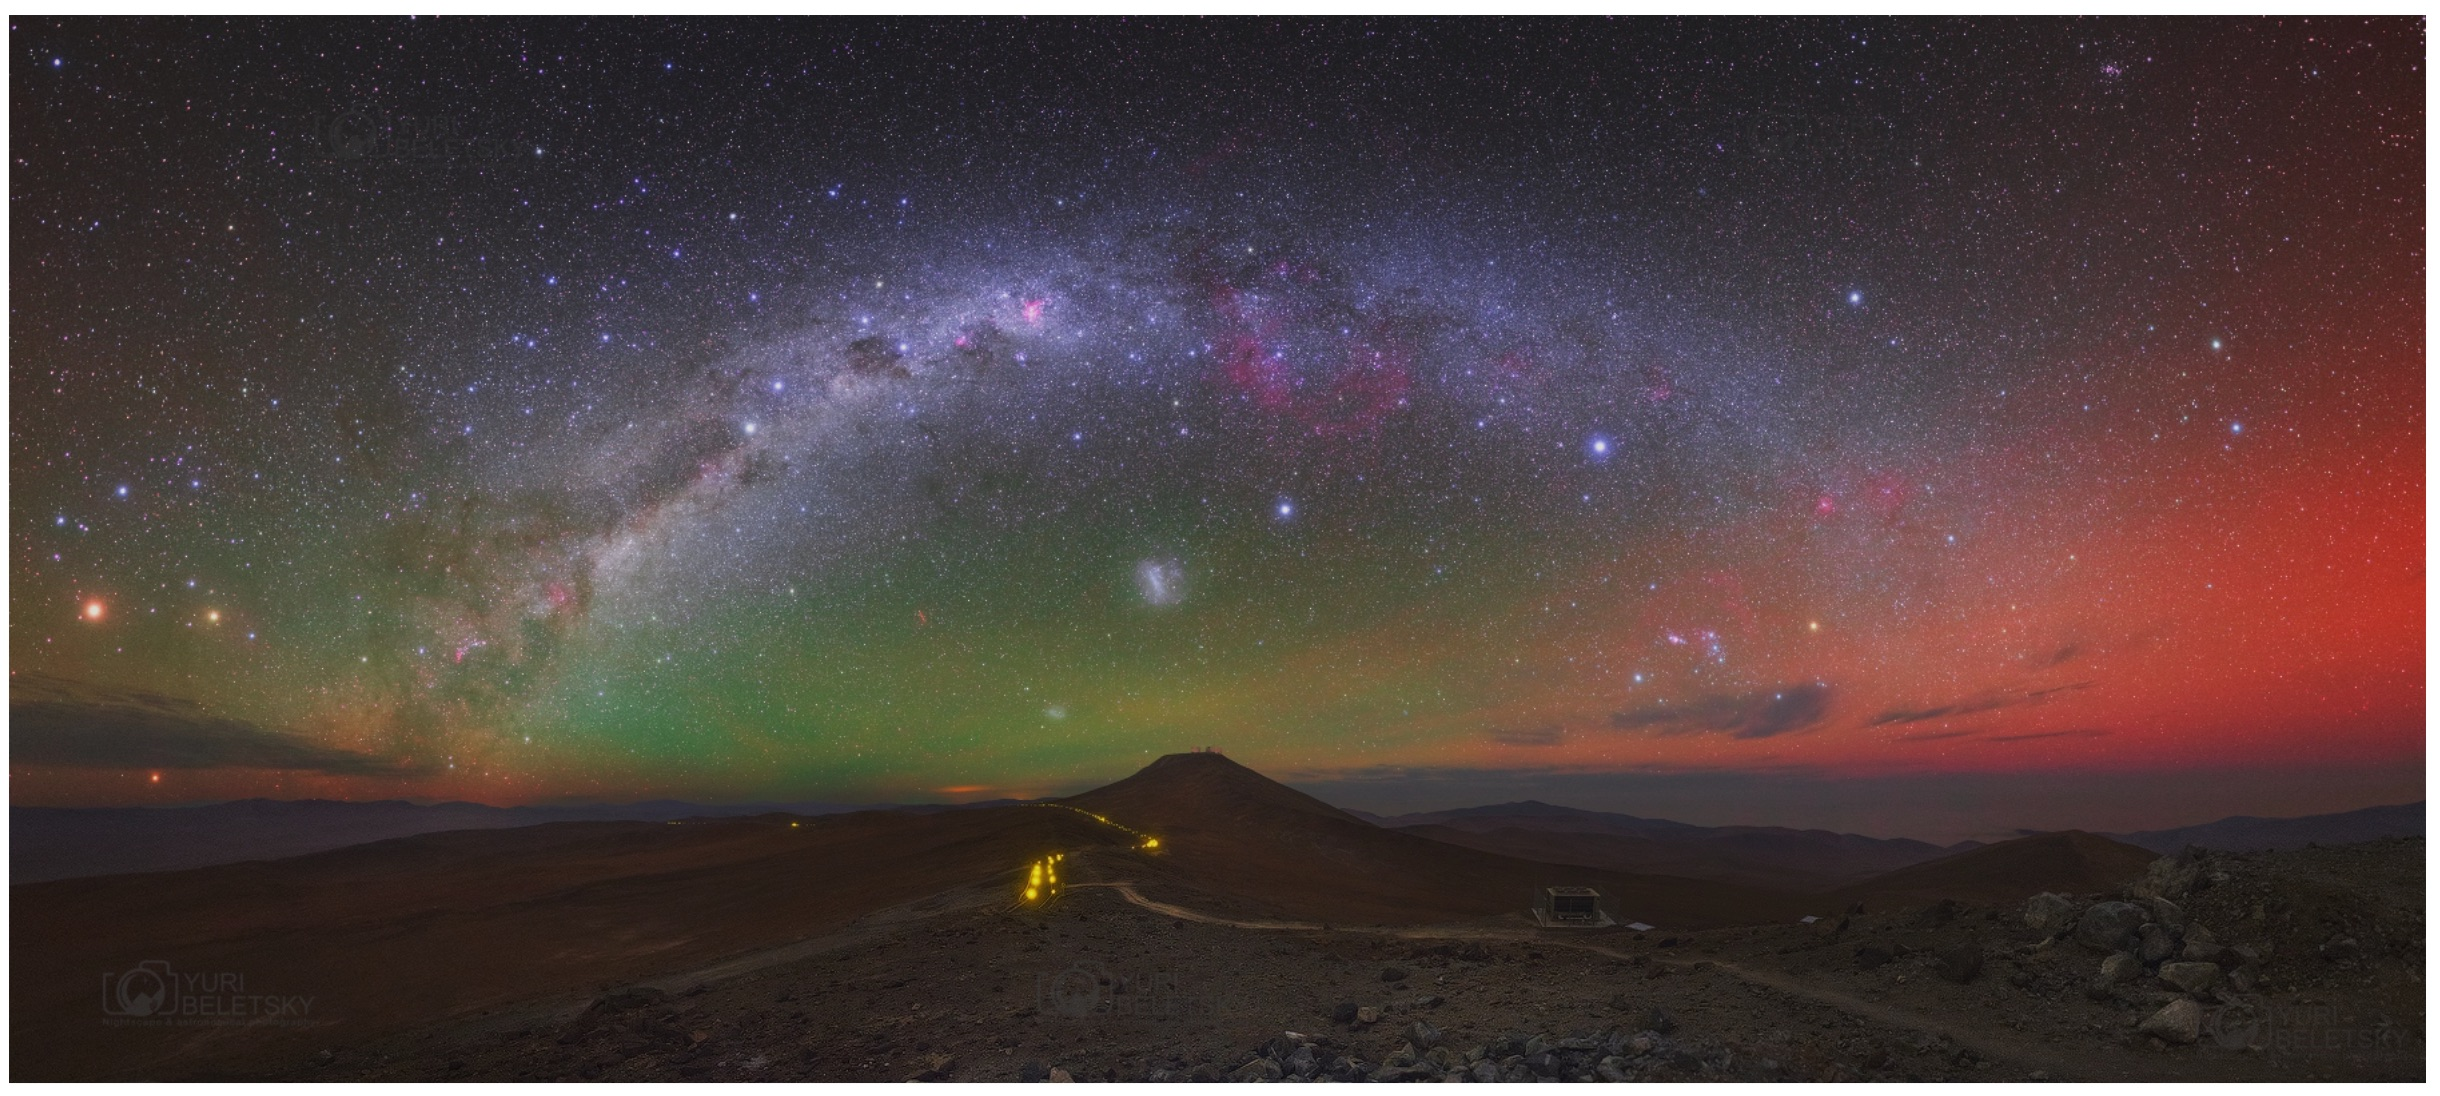
\includegraphics[width=1.0\textwidth]{milkyway.jpg}
\vspace{1.0in}

\huge
LSST Stars, Milky Way, and Local Volume Science Roadmap
\linebreak
\linebreak
\normalsize
{\bf Version v1.0}
\linebreak
{\bf Date: \today}
\end{center}

\pagebreak

\begin{table}[h]
\caption{Change Record}
\begin{center}
\label{tab:changerecord}
\begin{tabular}{|l|l|l|l|}
\hline 
\textbf{Version} & \textbf{Date} & \textbf{Description} & \textbf{Owner name} \\
\hline 
v1.0 & 20 November 2019 & Start of major rewrite & Peregrine McGehee \\
v0.1 & 19 June 2019 & Ingest of SWG roadmaps & Peregrine McGehee \\
\hline 
\end{tabular}
\end{center}
\end{table}

\pagebreak


\tableofcontents

\pagebreak

\section{Executive Summary}

The Large Synoptic Survey Telescope (LSST) is an 8.4-m dedicated survey telescope with a 3.2 Gigapixel camera under construction by the US National Science Foundation and the US Department of Energy. Construction of the camera is managed by the SLAC National Accelerator Laboratory, while the LSST observatory is under construction on its mountain-top site at Cerro Pachon, Chile. Work toward meeting the LSST science goals is being carried out by the LSST Science Collaborations.

The Stars, Milky Way and Local Volume Collaboration has the overarching goals of understanding the accretion history and structure of the Milky Way and the Local Volume, and the fundamental properties of stars within 300 pc of the Sun. These are also some of the main science drivers of both the telescope and the survey design of LSST, which will have unprecedented capability in the faint time domain.


\section{Introduction}

Guided by community-wide input, the LSST is designed to achieve multiple goals in four main
science themes: Taking an Inventory of the Solar System, {\bf Mapping the Milky Way}, Exploring the
Transient Optical Sky, and Probing Dark Energy and Dark Matter. These are just four of the many
areas on which LSST will have enormous impact, but they span the space of technical challenges
in the design of the system and the survey and have been used to focus the science requirements.


Encoded in the structure, chemical composition and kinematics of stars in our Milky Way is
a history of its formation. Surveys such as 2MASS and SDSS have demonstrated that the
halo has grown by accretion and cannibalization of companion galaxies, and it is clear that
the next steps require deep wide-field photometry, parallax, proper motions, and spectra to
put together the story of how our Galaxy formed. LSST will enable studies of the distribution of 
numerous main sequence stars beyond the presumed edge of the Galaxy?s halo,
their metallicity distribution throughout most of the halo, and their kinematics beyond the
thick disk/halo boundary, and will obtain direct distance measurements below the hydrogen burning limit for a representative thin-disk sample. 
LSST is ideally suited to answering two
basic questions about the Milky Way Galaxy: What is the structure and accretion history of
the Milky Way? What are the fundamental properties of all the stars within 300 pc of the
Sun?


LSST will produce a massive and exquisitely accurate photometric and astrometric data set.
Compared to SDSS, the best currently available optical survey, LSST will cover an area more
than twice as large, using hundreds of observations of the same region in a given filter instead
of one or two, and each observation will be about two magnitudes deeper. LSST will detect
of the order 1010 stars, with sufficient signal-to-noise ratio to enable accurate light curves,
geometric parallax, and proper motion measurements for about a billion stars. Accurate
multi-color photometry can be used for source classification (1\% colors are good enough to
separate main sequence and giant stars, Helmi et al. 2003), and measurement of detailed
stellar properties such as effective temperatures to an rms accuracy of 100 K and metallicity
to 0.3 dex rms.

To study the metallicity distribution of stars in the Sgr tidal stream (Majewski et al. 2003)
and other halo substructures at distances beyond the presumed boundary between the inner
and outer halo ($\sim$30 kpc, Carollo et al. 2007), the coadded depth in the $u$ band must reach
$\sim$24.5. To detect RR Lyrae stars beyond the Galaxy?s tidal radius at $\sim$300 kpc, the s
ingle visit depth must be $r\ sim $24.5. In order to measure the tangential velocity of stars to an
accuracy of 10 km s$^{?1}$
at a distance of 10 kpc, where the halo dominates over the disk, proper
motions must be measured to an accuracy of at least 0.2 mas yr$^{?1}$.

The same accuracy follows
from the requirement to obtain the same proper motion accuracy as Gaia (Perryman et al.
2001) at its faint limit ($r \sim$ 20). In order to produce a complete sample of solar neighborhood
stars out to a distance of 300 pc (the thin disk scale height), with 3$\sigma$ or better geometric
distances, trigonometric parallax measurements accurate to 1 mas are required. To achieve
the required proper motion and parallax accuracy with an assumed astrometric accuracy of
10 mas per observation per coordinate, approximately 1,000 observations are required. This
requirement on the number of observations is close to the independent constraint implied by
the difference between the total depth and the single visit depth.



\subsection{Science Collaboration Structure}
 
Our collaboration is organized into 7 Working Groups, each of which reflects a core scientific area being worked on by collaboration members. All collaboration members belong to at least one Working Group, and in early 2013, each Working Group was charged with creating a brief roadmap that highlights technical and scientific challenges that must be worked through to conduct our science with LSST. These roadmaps have been distilled into a list of active priorities, and the ongoing work tab gives a few examples of action items that collaboration members are actively pursuing.


Working Groups \& Leads:
\begin{enumerate}
\item The Solar Neighborhood: Adam Burgasser \& Todd Henry, lsst-milkyway-low@lsstcorp.org
\item Star Clusters: Kevin Covey \& Jay Strader, lsst-milkyway-sc@lsstcorp.org
\item The Galactic Bulge: Will Clarkson \& Victor Debattista, lsst-milkyway-bulge@lsstcorp.org
\item Galactic Structure and ISM: Peregrine McGehee, lsst-milkyway-struct@lsstcorp.org
\item Magellanic Clouds: Knut Olsen, lsst-milkyway-mc@lsstcorp.org
\item Near Field Cosmology: Marla Geha \& Carl Grillmair, lsst-milkyway-nfc@lsstcorp.org
\item Variable Stars: David Ciardi, lsst-milkyway-var@lsstcorp.org
\end{enumerate}

\subsubsection{The Solar Neighborhood}

Key target populations:
\begin{itemize}
\item{Solar 
neighborhood: classically d $<$ 10-25 pc, extend to $\sim$100 pc in LSST era}
\item{Young 
stars: clusters, moving groups \& associations }
\item{Old 
stars: subdwarfs, thick disk and halo objects, globular clusters (??) }
\item{Brown 
dwarfs: $<$0.07 Msun, including free-floating planets }
\item{White 
dwarfs (and other remnants?) }
\item{Binaries 
and higher order multiples: q $>$ 0.1, resolved and unresolved}
\item{Low 
mass companions: q $<$ 0.1, resolved and unresolved }
\end{itemize}


\subsubsection{Star Clusters}

Star clusters are a critical component of many of the science goals listed in the LSST Science Book (Ivezic et al. 2010). They offer unique environments where stars with a range of masses but similar ages and chemical compositions can be found. One class of studies aims to leverage these relatively simple stellar populations to understand the dependence of the stellar mass function and stellar evolution on metallicity and age (e.g., Sec. 6.5-6.6, 6.9-6.11; LSST Sci. Book). Their known properties and distances also motivate calibration work on many kinds of variable stars and transients (e.g., Sec 8.9; LSST Sci. Book). 

A separate class of studies is focused on using star clusters to trace the star formation history, chemical evolution, and galactic structure of the Milky Way, nearby galaxies (including the Magellanic Clouds), and even more distant galaxies extending beyond the Local Volume (e.g., Sec. 6.2-6.3, 6.6, 7.2, 7.3, 7.8, 7.10, 7.11; LSST Sci Book). 

\subsubsection{The Galactic Bulge}

These are kept deliberately broad at this stage (see Section 7 for more information), but point to the unique strengths of the Bulge as a test-case for Galaxy formation models: 
\begin{enumerate}
\item Detailed balance of populations as traced by morphology, chemistry, kinematics and distance 
\item The present-day mass distribution of the inner Milky Way as traced by Bulge star motions 
\item Wide-field examinations of other sub-populations and objects of interest. 
\end{enumerate}

\subsubsection{Galactic Structure and ISM}

{\bf Nothing!}

\subsubsection{Magellanic Clouds}

The LMC and SMC are the nearest large galaxies to the Milky Way and represent  fundamental testbeds for investigations related to many stellar astrophysical topics,  from studying the star formation process, to the physics of variable star populations,  to the physics of galaxy interactions, and to calibrating the cosmological distance  scale.    

The Clouds are some of the bestGstudied galaxies in the Universe, yet nevertheless  consistently have the power to surprise.  A recent surprise is that the Clouds, which  have long been thought of as closely bound satellites of the Milky Way, appear to be  on first infall, or at most have made a small number of close passages, based on  proper motion measurements (Kallivayalil et al. 2006a,b; Besla et al. 2007, Piatek et  al. 2008, Kallivayalil et al. 2013).  We have also seen evidence that the LMC has  accreted a significant mass in stars from the SMC (Olsen et al. 2011), which may  indicate that the LMC and SMC collided directly with each other ~100 Myr ago  (Besla et al. 2012), a discovery that relied on the proper motion work.  The HI tidal  streamers that connect the LMC to the SMC and Magellanic Stream are kinematically  linked to the accreted SMC stars, and thus may have formed in this collision; the  streamers converge on the location of 30 Doradus in the LMC (Nidever et al. 2008),  indicating that 30 Doradus may be an interactionGinduced star formation event.   Moreover, the stellar debris left behind by the SMC could naturally explain the  microlensing event rate (Besla et al. 2013) seen towards the LMC by e.g. MACHO and  OGLE.  

The Magellanic Clouds are also now known to extend to much larger radius than  known before, through several pencilGbeam studies.  Majewski et al. (2009) found  spectroscopicallyGconfirmed KGgiant LMC stars at large distances (R $\sim$ 22 or 19 kpc),  while Saha et al. (2010) found that the LMC exponential disk extends past 12 disk  scale lengths.  In the SMC, Nidever et al. (2011) traced K giants to $\sim$11, with  possible evidence for a stellar halo.  These studies are based on exploration of 1  of the relevant area of sky.  There is thus a vast area that remains to be explored for  hidden Magellanic Clouds structure, with implications both for understanding the  history of the Clouds and the formation of the Galactic halo.   

There are many other recent exciting discoveries in the Magellanic Clouds that have  not been mentioned here.  The point of mentioning the few above is to demonstrate  that 1) in the Clouds, astrophysical problems are often connected across broad areas  of study, 2) Magellanic Cloud populations cover a very large area of sky, and 3)  highly precise measurements, such as produced by the work on LMC and SMC  proper motions, have the power to fundamentally alter accepted understanding.  

\subsection{Cross-collaboration initiatives}

\subsubsection{Variable Stars}

The science of variable stars is effectively split between the Transients \& Variable Stars ( TVS) Work- ing Group and the Stars, Milky Way, and Local Volume (SMWLV) Working Group. This subgroup will serve as a bridge between the two Working Groups to maintain a focus on this important scientific area. 

{\bf Collaboration with Transients \& Variable Stars Working Group:}
One of the key questions about our subgroup is what science will be primarily covered by the SMWLV group versus the TVS group. In general, extragalactic transients like supernovae and GRBs will be dealt with by the TVS. That still leaves eclipsing, rotational, pulsating, and flaring stars. So far most of the work on pulsating stars (i.e. RR Lyrae) has taken place within the TVS group, and so we will only briefly discuss such variables in this roadmap. However, we should remain careful to prevent any scientifically interesting variable type from falling through the cracks between the two working groups. 

{\bf Classification of Variables:}
A very broad issue that both Working Groups (TVS and SMWLV) will have to deal with is the nature of LSST classification. No science can be accomplished in the area of variable stars unless we resolve the question of how the LSST pipeline will classify the enormous variety of variable stars, and at what level. 
Will stars be simply identified as Variable or Not Variable based on some confidence level of a given statistical test? Or will the classification go deeper, into identifying stars as periodically versus non- periodically variable, or even further into sorting them into specific categories, such as eclipsing, pulsating, etc.? This is arguably the single most important question for variable star science with the LSST. There are existing efforts to approach this problem, including the EB Factory project (Stassun et al. 2013) at Vanderbilt University1, and efforts led by Josh Bloom (Bloom et al. 2012). However those efforts will have to be more fully developed for the variable star science goals of LSST. Current variability surveys such as the Palomar Transient Factory and the Catalina Sky Survey offer precursor data sets that can be used for testing classification methods. 

\subsubsection{Near Field Cosmology}

Dark matter constitutes roughly 85\% of the matter density of the Universe, and represents a critical gap in our understanding of fundamental physics. Despite these extensive experimental efforts, the only robust, positive empirical measurement of dark matter continues to come from cosmological and astrophysical observations. The Large Synoptic Survey Telescope (LSST) offers a unique avenue to attack the dark matter problem. Our group seeks to identify and pursue scientific avenues to utilize LSST to help us understand the fundamental physics that governs dark matter. Specifically, we hope to identify the fundamental constituents of dark matter (e.g., new fundamental particles, fields, or compact objects) and to characterize the properties of these constituents (e.g, mass, temperature, self-interaction rate).
A major initiative in the study of dark matter has been formed with the LSST Dark Energy Science Collaboration [DESC], see
{\it https://lsstdarkmatter.github.io/index.html}.

The LSST Near Field Cosmology subgroup focuses on using stellar substructure throughout the Milky Way
 and Local Volume as a probe of the underlying CDM cosmology.  
This includes searches for dwarf galaxies, tidal streams and other coherent features in 
phase space using the properties of individual stars. 
Examples include searches for ultra-faint galaxies based on overdensity of main sequence stars, 
searches for substructure using RR Lyrae variables, or searches for moving stellar groups using proper motions. 

Searches for Milky Way substructure will allow critical new constraints in several areas. 
A more complete census and map of the distribution of satellites around the Milky Way sheds 
light both on the formation of satellite systems and the nature of dark matter halos that are 
able to host such low-mass galaxies.
 Finding tidal debris beyond 100 kpc and out to the virial radius of the Milky Way will open a 
window on the more recent accretion history of the Galaxy, as well as the accretion of objects 
on more radial orbits in particular. 
Debris in the outer Galaxy also promises a powerful new probe of the mass 
distribution around the Milky Way in regions of a dark matter halo that have been largely 
unexplored for any galaxy in the Universe. 

\subsubsection{Education \& Public Outreach}

{\bf Needs text}


\section{Key Science Analyses}


\section{Enabling Analysis}


\section{Pipelines and Computing Infrastructure}


\include{datasets}
\include{deliverables}
\section{Research and Development}

\subsection{Introduction to Collaboration R\&D Priorities}

A number of priorities have been defined with the SMWLV collaboration, here we give an overview. The details of these issues are spelled out in further sections.

{\bf These are from the milkyway website, we have an updated set from the 2019 PCW breakout sessions.}

\begin{enumerate}

\item{Crowded field photometry/astrometry (Example action items: DECam precursor studies of Galactic bulge/plane to estimate the source density as a function of position; Use ImSim pipeline to create synthetic images of crowded fields and test LSST?s astrometry and photometry on resultant CMDs).}

\item{Star-galaxy separation (Example action items: HST archival project to generate a point source/extended source truth table; Use of SMASH survey of Magellanic Clouds to empirically benchmark impact of unresolved galaxies on LSB structure mapping; Multi-color deep wide-field surveys of known LSB systems to test star-galaxy separation algorithms; Use ImSim input catalog to test star-galaxy separation algorithms).}

\item{Photometric metallicity calibration (Example action items: Assemble relevant spectral and photometric datasets. Compare to existing efforts from SDSS, including Ivezic metallicities for FGK stars, and Mann, Lepine and West calibrations for M dwarfs. What are the ranges in mass/color where these relations are valid? Extend these applications to LSST, assuming a LSST-SDSS transformation is robust. Using archival spectra or PanSTARRS data, test how y-band photometry can improve the photometric metallicity estimate. How can time-series information be used to improve metallicity estimates (e.g., Miller, Richards, Bloom et al).}

\item{y4 filter calibration (Example action items: Ground based/space based y4 investigations; Can PanSTARRS experience be leveraged for y-band calibration? How does varying the water column change the spectral response. Simulate the effect of a varying water column on the y4 filter using existing spectra of FGKM stars.).
Cadence Planning (Example action items: Build the case for Magellanic Clouds cadence; Develop the science and technical case for MW disk and bulge cadence; Develop and test cadence metrics for astrometry).}

\item{Stellar variability classification (Example action items: Define classification metrics required for your specific science goals, see example in Near Field Cosmology roadmap; Develop light curve classifiers + period finders and test on existing datasets [e.g. LINEAR]; coordinate with Transients science collaboration and tools from EB factory general purpose light curve classifier and intelligent period finder; DECam Bulge survey).}

\item{Subgroup specific technical needs (Action items: As defined by individual collaboration members and Working group leads, e.g. photometry of nebulae.).}

\item{Theoretical predictions for LSST Milky Way science (Example action items: As defined by individual collaboration members and Working group leads, e.g., simulations that make predictions for LSST; coordinate with Justin Read?s Gaia challenges).}

\end{enumerate}


\subsection{Update from 2019 PCW}

Here are some important updates from the LSST Project and Community Workshop held earlier this month in Tucson:

\begin{enumerate}

\item{Crowded Field Photometry: The project is making a plan to process crowded stellar fields with a special deblender, i.e., a DAOPhot-like system integrated into the LSST DM pipeline, and not the same deblender being developed to deal with galaxies at high galactic latitude. They believe an in-house DM solution has significant advantages over using existing external codes. A document (plan) explaining their approach is expected around September 1. We will have two months to provide feedback. [See Task Forces below]}

\item{New "Task Forces" for 2019-2020:  We had a meeting of SMWLV members. We decided to form a number of task forces which have a defined mission and finite lifetime.  A number of volunteers, but we badly need more.}

\end{enumerate}

\subsubsection{Proposed task forces}

CADENCE SIMULATIONS: Tasks: Review existing cadence metrics and identify new metrics. Work with LSST MAF group to implement metrics. Complete this within 4 months. After feedback from our collaboration, analyze results of simulations.  Volunteers: Olsen, Clarkson, Leo, Marcio,

CROWDED FIELD: Read and comment on DM crowded field photometry plan by November. Volunteers: Clarkson, Nidever,Adriano Pieres 

COMMISSIONING: Review LSST official document on commissioning tests. Lead discussion of tests that we feel are missing. Identify participants to directly participate in commissioning, early access sprints, data preview sprints. Many timescales, but reading and planning can occur in next six months. We anticipate most work is in 2020-2021. Volunteers: Olsen. 

ASTROMETRY: Investigate Differential Color Refraction (DCR). Identify data and develop proposal if necessary. Volunteers: D. Monet, Jullio Camargo

CALIBRATION: Investigate water bands and calibration (y) filter. New calibration data expected in spring 2020, so start then. (Should also reach out to supernovae people). Volunteer: Pat Boeshaar.

DATA CHALLENGE: Plan sprint or data challenges of our own to do science. Volunteer: Clarkson.

Other task forces are welcome. The first three were considered the most urgent and important.  Please volunteer! 


\subsubsection{Crowded field photometry}

\subsubsection{Star-galaxy separation}

\subsubsection{Photometric metallicity calibration}

\subsubsection{y4 filter calibration}

\subsubsection{Stellar variability calibration}

\subsubsection{Subgroup specific technical needs}

\subsubsection{Theoretical predictions for LSST SMWLV science}








\section{Appendices}



\section{References}



\bibliographystyle{apj}
\begingroup
    \setlength{\bibsep}{0pt}
%%    \setstretch{1}
    \bibliography{references}
\endgroup




The following sections are copies of the material created by each working group during the 2013-era 
roadmap initiative.


\section{LSST Phase 1 Science Roadmap - Bulge subgroup v1.0, August 2013}

Summary: This is version 1.0 of the LSST Bulge Science Phase 1 Roadmap. The Phase I document should identify the technical and scientific challenges for LSST Bulge work (without going overboard on the science) and to start to identify tasks for collaboration members in order to overcome these challenges on a timescale of a few years. 

Based on input from the Bulge subgroup, we have identified a number of technical issues that are important to Bulge science with LSST. We also highlight some suggested investigations - mostly based on simulation and archival work - that we believe would allow LSST to become a unique machine for conducting scientific discovery about the Milky Way Bulge. This document is organized as follows: 
\begin{enumerate}
\item Summary of Bulge LSST Science goals and match to LSST capabilities
\item Main technical issues these goals bring up 
\item Investigations that should be performed / questions to answer at this stage. 
\item Questions already arising for LSST development team 
\item References cited 
\item Figures 
\item Appendix: more detail about the Bulge LSST Science goals 
\end{enumerate}

A note on editing: Feel free to email either the subgroup leads (Will Clarkson and Victor Debattista; 
wiclarkson@gmail.com and vpdebattista@gmail.com ) or the mailing list (lsst-milkyway-bulge@lsstcorp.org ) with suggested edits. 

\subsection{Overview of LSST Bulge science goals}

These are kept deliberately broad at this stage (see Section 7 for more information), but point to the unique strengths of the Bulge as a test-case for Galaxy formation models: 
\begin{enumerate}
\item Detailed balance of populations as traced by morphology, chemistry, kinematics and distance 
\item The present-day mass distribution of the inner Milky Way as traced by Bulge star motions 
\item Wide-field examinations of other sub-populations and objects of interest. 
\end{enumerate}

\subsection{Match to LSST capabilities}
If the numbers in Ivezic et al. (2008), the Science Requirements Document (SRD) and the LSST Science Book are realized for the Bulge populations of interest, these three science goals should be within the capabilities of LSST. For reference, those numbers are: 
\begin{itemize}
\item Relative photometry: 5 mmag per-measurement rms (g,r,i), perhaps 50\% larger for u,z,y (SRD Table 14) 
\item Absolute photometry: 10 mmag per-measurement rms, color zero-points accurate to 5 mmag rms (SRD 
Tables 15, 16) 
\item Relative astrometry: 10-15 mas per-measurement rms depending on separation (SRD Table 18) 
\item Absolute astrometry: 50 mas per coordinate (SRD Table 20) 
\item Pixel-scale and seeing: Pixel-scale $\le$ 220 mas; at airmass 2, 
seeing-error 0.5 arcsec ($\gtrsim$ 2.3 pix; SRD 
Tables 10,11) 
\item Shortest possible exposure time: 5 sec, stretch-goal 1 sec (SRD Table 8) 
\item{At r=20, predicted performance when measurements are combined over the 10-year baseline survey:
\begin{itemize} 
\item Proper motion accuracy: 0.14 mas/yr, Photometric error 0.005 mag (single-visit), 0.003 mag (stack) 
\item These numbers come from from Table 6.6 and Figure 6.26 on Pages 193-195 of the LSST Science Book, v2. 
\item Note that the 10-year baseline survey is likely to be rather more generous than Bulge observations (by a factor of several - see Section 2.3). 
\end{itemize}
}
\item{For context, here are approximate apparent magnitudes for bulge populations of interest: MSTO roughly r$\sim$19.5 (r-band absolute magnitude about 4.0, plus distance and extinction), Red Clump giants roughly r$\sim$7.0 Note, however, that variations in the line of sight distance and extinction significantly broaden the observed distribution (X-shape alone leading to variation by 0.5 magnitudes or more; e.g. Saito et al. 2011). }
\end{itemize}
However, most of the Bulge populations of interest are more crowded than the baseline LSST survey to which the 
above numbers apply (Section 2.1 and Figure 1). 
While a seeing-limited large-scale survey like LSST is likely to be transformative for Bulge science, to reach these science goals we do need to understand how the LSST performance numbers change towards the Bulge, and what strategy will successfully overcome any limitations of the current reduction plans. 

\subsection{Leading Technical Issues}

\subsubsection{LSST as complementary to Gaia towards the inner MW}
LSST is supposed to smoothly extend the error-vs-magnitude curve of Gaia to fainter magnitudes (Ivezic 2008). Here are summary numbers for GAIA (de Bruijne et al. 2012 and Brown 2013), which are a bit more generous than Reyle et al. (2008; Figure 1). 
\begin{itemize}
\item Gaia Astrometry OK up to about 1 million stars / sq. deg., corresponding to about 278 stars per square arcmin. 
\item Gaia Photometry OK up to about 200 stars per square arcmin 
\item Gaia Spectroscopy OK up to about 10 stars per square arcmin 
\item Brown (2013) indicates $\sim$800 stars / sq. arcmin “can be dealt with” - what does this mean for actual 
precisions in this regime? 
\end{itemize}

For non-crowded regions (e.g. Science Book p193-195), LSST’s precision starts to exceed Gaia’s 
precision at r$\sim$~19.5 or so, comparable to the MSTO and sufficient to well-characterise 
red-clump giants already. 
However, this is unlikely to be realized in 
practice due to crowding; the GAIA - LSST handover magnitude may be somewhat brighter. 
\begin{itemize}

\item Gaia performance: What will the true performance of Gaia be towards the MW Bulge in reality? See e.g. Figure 1. 
\item Gaia/LSST magnitude boundary: In crowded fields, at what apparent magnitude will Gaia’s performance degrade and LSST be expected to “take over?” Is this transition magnitude fainter than, say, the fainter Red Clump Giants (RGC)s in most Bulge fields? 
\item Gaia’s observing strategy: For those objects within Gaia’s magnitude range of accuracy, how does Gaia’s observing cadence map onto the science goals for LSST Bulge work? 
\item Gaia and LSST in overlapping brightness ranges: For the brightness interval in which Gaia and LSST overlap in coverage, what will LSST add to those objects? Should observations in this overlap magnitude range be scheduled for cross-calibration, in the crowded fields towards the Bulge? 
\end{itemize}

\subsubsection{Crowded-field Photometry and Astrometry}
 This was perhaps the most common technical response in the Survey amongst MWLV members! 
The performance specifications in the Ivezic et al. (2008) survey document and the SRD, are for regions that are not too crowded, although it does not appear that 
the collaboration has yet reached official consensus on what "crowded" really means. At the moment, the rule of thumb appears to be 
about 200 stars per square arcmin. 
This limit is reached before the Main Sequence Turn-Off in many fields 
towards the bulge (Figure 1).
 
Thus, reaching the MSTO will likely require pushing LSST's photometry and 
astrometry software to regions that are much more crowded than LSST’s existing analysis stack was built to handle. Arising from this: 
\begin{itemize}
\item What measurement approaches will work best for LSST Bulge crowded fields? 
\item{Is rapid turnaround important for LSST Bulge photometry, or is a careful, if slower, analysis (taking, say, 
a few weeks to process) appropriate? }
\item Is rapid turnaround important for LSST Bulge astrometry? 
\item{In what mode will crowded-field work be performed? Do we require optional tools that would be run on 
specific small regions, or is it essential instead to produce the photometric and astrometric catalog for 
all regions observed, no matter how crowded? }
\item{What is the limiting depth required by the LSST Bulge science goals? To what source density (e.g. stars 
per square arcmin) does this correspond in real Bulge fields? }
\item{Conversely, if we assume the baseline analysis software that will deliver photometry and astrometry for 
regions $<$ 200 stars / sq. arcmin, how does this impact the Science Goals? See e.g. Figure 1 in Section 6 
below.}
\item{If any science goals are precluded under the baseline scenario, does their resurrection deliver science of 
sufficient import to justify the extra effort developing crowded-field analysis tools? }
\item{
The LSST planning software already includes sophisticated tools to simulate stellar populations in the 
inner MW (its crowding predictions towards the plane were used to set the galactic latitude limits for the main LSST survey). How well do the predictions of these tools match reality? Are their predictions too conservative? }
\item{One survey respondent recommended that astrometry not be treated as an afterthought, but be built in to analysis tools as a key requirement. }
\end{itemize}

\subsubsection{Observation setup (including total time, saturation issues)}
How do the different science goals interact with each other when designing observations? Are some science cases excluded by others? 

\begin{itemize}
\item{Total observing time: Based on a quick query of OpSim (performed in June 2012), bulge fields were slated to receive ~one fifth the number of pointings per field when compared to the baseline survey (Figure 2). Assuming those numbers are still current, now is the time to advocate for a more suitable strategy. In particular: 

\begin{itemize}
\item{Lower number of exposures per field is probably unimportant for deep stacks since the crowding is higher than baseline anyway. }
\item{ However, for investigations requiring multiple exposures whatever the depth (e.g. proper motions, monitoring variable-object standard candles), the reduced total number of observations might prevent the desired science goal being reached. }
\item How should observations be distributed along the total time allocation to maximize the science? 
\item How many pointings per object are needed for a given science case? 
\item Is there a strong enough case to request a larger total allocation time? 
\item{Saturation issues: What range of exposure times will allow both the bright and faint objects to be 
covered in the same campaign? What is the observing duty cycle as a function of exposure time? At what 
(if any) instrumental magnitude do persistence effects set in? }
\item{
Cadence: How do the cadence requirements for the different science cases interact with each other? For 
example, can variable-object standard candles with very long periods (hundreds of days or longer) be monitored in an observing program that also seeks short-period variables? In this example, if (say) a logarithmic cadence strategy is adopted, does this preclude other science? }
\item{What happens if the total allocation for Bulge science is reduced? Do we need to produce a contingency plan in this case? }
\item{Extinction and filter choice: Will extinction-correction rely on cross-matching to catalogs at other wavelengths? Or, does the requirement to correct for extinction drive a minimum number of filters for every observation? }
\item{Astrometry and filter choice: The Science book (Section 3.7) seems to suggest that the (r, i) filters will be best for astrometry. To pursue bulge astrometry, should a separate set of observations in a smaller number of filters be taken? }
\end{itemize}
}
\end{itemize}

\subsubsection{Calibration and calibration products}
\begin{itemize}
\item What calibrations do we (the investigators) need to conduct our own specialized analyses of favorite 
regions? 
\item How will calibration products be made available to the community? 
\item{For how long and in what format will supporting observational telemetry (e.g. telescope temperature, 
observed seeing, etc.) be maintained? WIll this be available to the investigator? }
\end{itemize}

\subsection{Investigations suggested for LSST Bulge science}
The above considerations suggest the following investigations. We are aware that in several cases this might be as quick as a literature or archive-search. 
\subsubsection{Simulation}
Baseline capability of LSST in crowded fields with the currently-planned measurement software: 
\begin{itemize}
\item{Simulate observations towards a variety of regions towards the Bulge, at a variety of exposure-times, 
with input properties of interest (e.g. variability, proper motion, extinction), and attempt to recover these using the existing software stack. }
\item{Use this to estimate random and systematic effects on photometric and astrometric completeness and precision as a function of the stellar crowding. }
\item{This dataset might already exist - were these simulations performed to set the Galactic Plane avoidance limits for the baseline survey already? }
\end{itemize}

\subsubsection{Simulation + Archive}
Science impact of crowding limit: Using crowding limits obtained from 4.1 above or otherwise, examine available source-catalogs towards the bulge to determine, under those crowding limits: 
\begin{itemize}
\item What is the region of avoidance with current LSST software, in galactic coordinates, as a function of magnitude? 
\item What stellar populations in and towards the bulge become unavailable using this limitation? 
\item What science does this preclude? 
\end{itemize}

\subsubsection{Simulation}
Observing strategy for saturated objects in crowded fields: 
\begin{itemize}
\item{Simulate observations for a well-chosen sample of fields towards the Bulge, at a range of exposure times 
from 1s to 15s, to estimate: 
\begin{itemize}
\item What range of exposure times is needed to attain high-precision measurements of the bright 
stars in the field of view? 
\item What artefacts are bright objects expected to produce in the longer exposures, and how can 
their effects be characterized and mitigated? 
\item How do measurement systematics vary with exposure time? 
\item What is the tradeoff between observing efficiency and exposure time? 
\end{itemize}
}
\end{itemize}

\subsubsection{Literature, Simulation, ground-based data}
Performance of existing crowded-field photometry and astrometry tools on likely LSST observations towards the Bulge: 
\begin{itemize}
\item How do existing crowded-field measurement techniques scale to LSST-like applications? 
\item{What scale of simulation is practical before LSST goes on-line? Can we expect to run a complete suite of 
imaging-sets under a variety of reduction strategies? }
\item{How do changes to analysis software fit in with the LSST software pipeline as it currently exists? }
\end{itemize}

\subsubsection{Simulation combined with existing data and archives): Fidelity of LSST’s simulation software applied to Bulge regions: }
\begin{itemize}
\item{Compare LSST simulation predictions with existing datasets towards the Bulge to determine how well these simulations reproduce actual data. }
\item{A large number of potential comparison datasets, from broad-shallow to narrow-deep}
\item{The ImSim/OpSim team might already be doing this... }
\end{itemize}

\subsubsection{(Simulation, literature, archives): Harder numbers for science requirements: }
\begin{itemize}
\item{
Use existing archives / literature to map figures of interest across the bulge region (e.g. number of stars 
per square arcminute down to a limiting depth as a function of apparent magnitude and color). Do this 
for several populations of interest (e.g. Red Clump Giants). }
\item{Modeling: To make further progress on (for example) mass models of the Bulge, what size of tracer-star 
sample is needed? }
\item{Modeling: Under the current best bulge models, what is the prediction of proper motion as a function of 
line of sight distance for sight-lines towards the bulge? What does this imply for proper motion precision requirements? }
\end{itemize}


\subsubsection{(Simulation): Observing strategy to best meet science goals: dithering, pointings}
\begin{itemize}
\item{Simulate observations with different dithering strategies to determine the best strategy under likely time 
allocations.}
\end{itemize}

\subsubsection{(Archive, Simulation): Appropriateness of existing catalogs for LSST Bulge operations: }
\begin{itemize}
\item{Determine to what extent successful observations require information from external catalogs to succeed. 
Determine how the quality of these catalogs changes over the Bulge, and thus what (if any) effect variation in external catalog quality will hinder science observations towards the Bulge. }
\end{itemize}

\subsubsection{Literature, personal communication): Complementarity to GAIA }
\begin{itemize}
\item{Find out the current best estimate for GAIA’s performance towards the Bulge. Do hard numbers exist from 
the GAIA team for what happens to GAIA’s astrometric and photometric precision in highly crowded regions? What did Brown (2013) mean by “[$\sim$800 stars/sq arcmin] can be dealt with”? }
\end{itemize}

\subsubsection{(Observation, archive): Precursor data }
\begin{itemize}
\item{Determine what precursor data already exists to answer the questions raised in this document. }
\item{As a sub-group, if necessary regions of parameter-space are NOT probed by these observations, 
determine a consensus plan to apply for further precursor data. }
\item{We want to avoid the situation where members of the LSST Bulge sub-group submit proposals 
that compete with each other for similar precursor data. }
\end{itemize}

\subsection{Questions and wishlist arising for those developing the LSST facility and its software}
\subsubsection{Existing simulations: }
\begin{itemize}
\item Improved knowledge desired on how to access simulated datasets. 
\end{itemize}

\subsubsection{Running custom simulations }
\begin{itemize}
\item What computer hardware is required to run LSST simulations? 
\item{What is the key factor determining the variation of time elapsed for a simulation on the same hardware 
-- the total number of sources, or something else? }
\item{Tutorials are desired on how to set up and run the simulation software. }
\end{itemize}

\subsection{Existing and planned analysis software }
\begin{itemize}
\item Tutorials on the Data Management system 
\item{Detailed understanding of the uncertainties (their production and propagation) through the LSST 
simulations and measurement routines }
\item{Tutorial on running the LSST pipeline on non-LSST data }
\item{What are the current capabilities of point-source software for LSST? What are its limitations (e.g. 
maximum array-size)? }
\end{itemize}

\subsubsection{External catalogs for LSST photometry }
\begin{itemize}
\item How reliant is LSST calibration on cross-matching to external catalogs? 
\item What capabilities for cross-matching with external catalogs, can we expect? 
\item{ Bulge regions may have more sources per square arcmin than typical for the baseline survey. How does 
the time required to crossmatch scale with catalog size? How are multiple possible matches handled? }
\end{itemize}

\subsection{References cited: }
%%\begin{verbatim}
%%1. Brown 2013: http://www.strw.leidenuniv.nl/~brown/gaia/gaia­dpac­overview.pdf 
%%2. de Bruijne et al. 2012: http://adsabs.harvard.edu/abs/2012Ap%26SS.341...31D 
%%3. Howard, C. D. et al. 2009 ApJ 702, L153 
%%4. Ivezic, Z. et al. 2008 http://arxiv.org/abs/0805.2366 
%%5. Nidever, D. L. et al. 2012 ApJ 755, L25 
%%6. Reyle, C. et al. 2008: http://arxiv.org/abs/0812.3743v1 
%%7. Saito, R. 2011 AJ 142, 76 
%%\end{verbatim}

\subsection{Figures }

\begin{figure}[h]
    \centering
    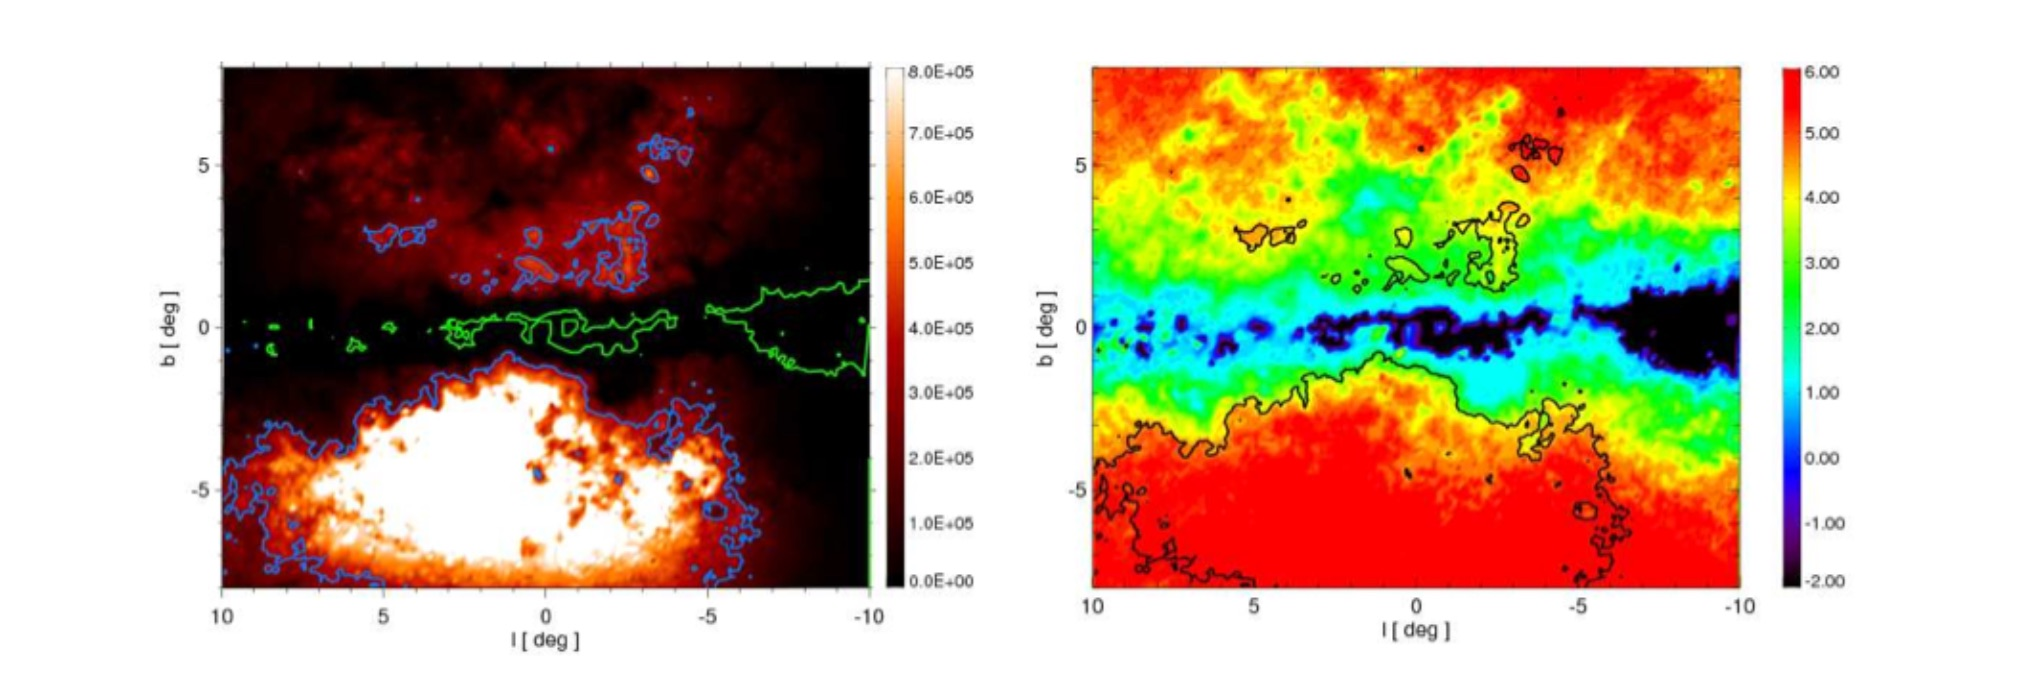
\includegraphics[width=1.0\textwidth]{bulge_fig1a.jpeg}
    \caption{\label{fig:bulge1a}
Figure 1a: This shows predictions of the Besancon model for the inner Milky Way, in the context of GAIA’s performance estimates as of 2008. The left-hand panels show spatial density (stars per sq. deg.), the right shows the absolute magnitude (in G-band, approx SDSS r) of stars just reached at their assumed limiting magnitude. This figure shows GAIA’s astrometric fields (the GRP and GBP instruments – limiting magnitude G=20). The blue contour shows the iso-density of 600,000 stars per square degree (167 stars per square arcminute, or a little less 
crowded than LSST’s baseline limit at present). The green contour shows the iso-density of 100 stars per square degree, or 0.028 stars per square arcminute. Notice that in G-band, it is the bright area away from the plane that is in the region of avoidance, not the dark area covering the plane itself. This is Figure 3 of Reyle et al. 2008. }
\end{figure}

\begin{figure}[h]
    \centering
    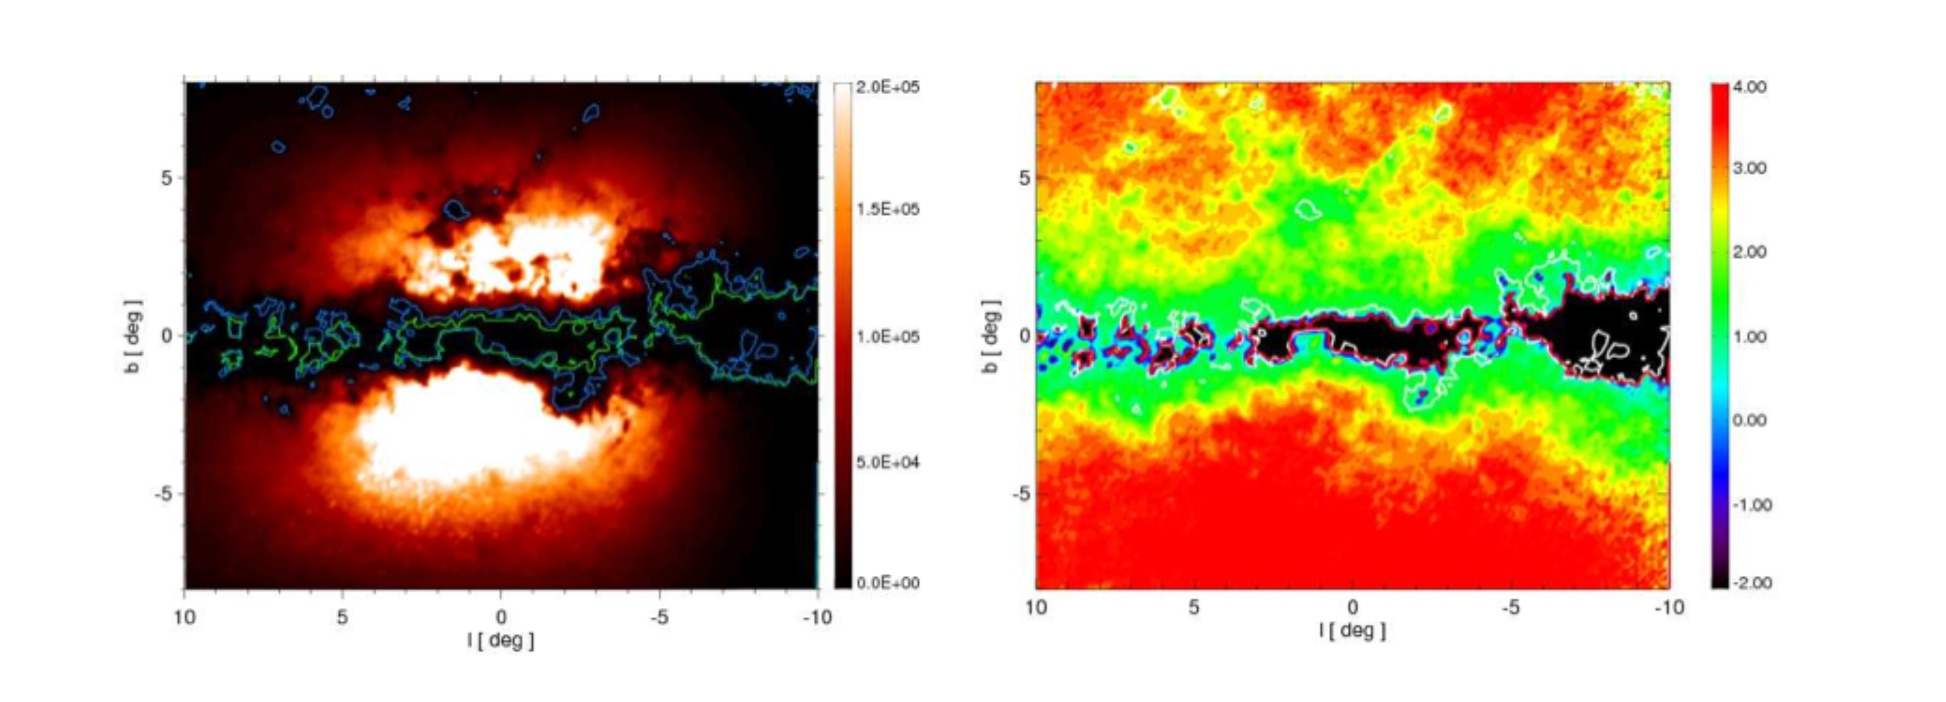
\includegraphics[width=1.0\textwidth]{bulge_fig1b.jpeg}
    \caption{\label{fig:bulge1b}
Figure 1b: As Figure 1a, this time for GAIA’s spectrometer (RVS). This instrument has limiting magnitude G=17 and a much more stringent crowding limit: 30,000 stars per square degree, or about 8.3 stars per square arcminute. With these performance numbers, only the very inner (extincted) plane is accessible to GAIA’s RVS spectrometer. This is Figure 4 of Reyle et al. 2008. }
\end{figure}

\begin{figure}[h]
    \centering
    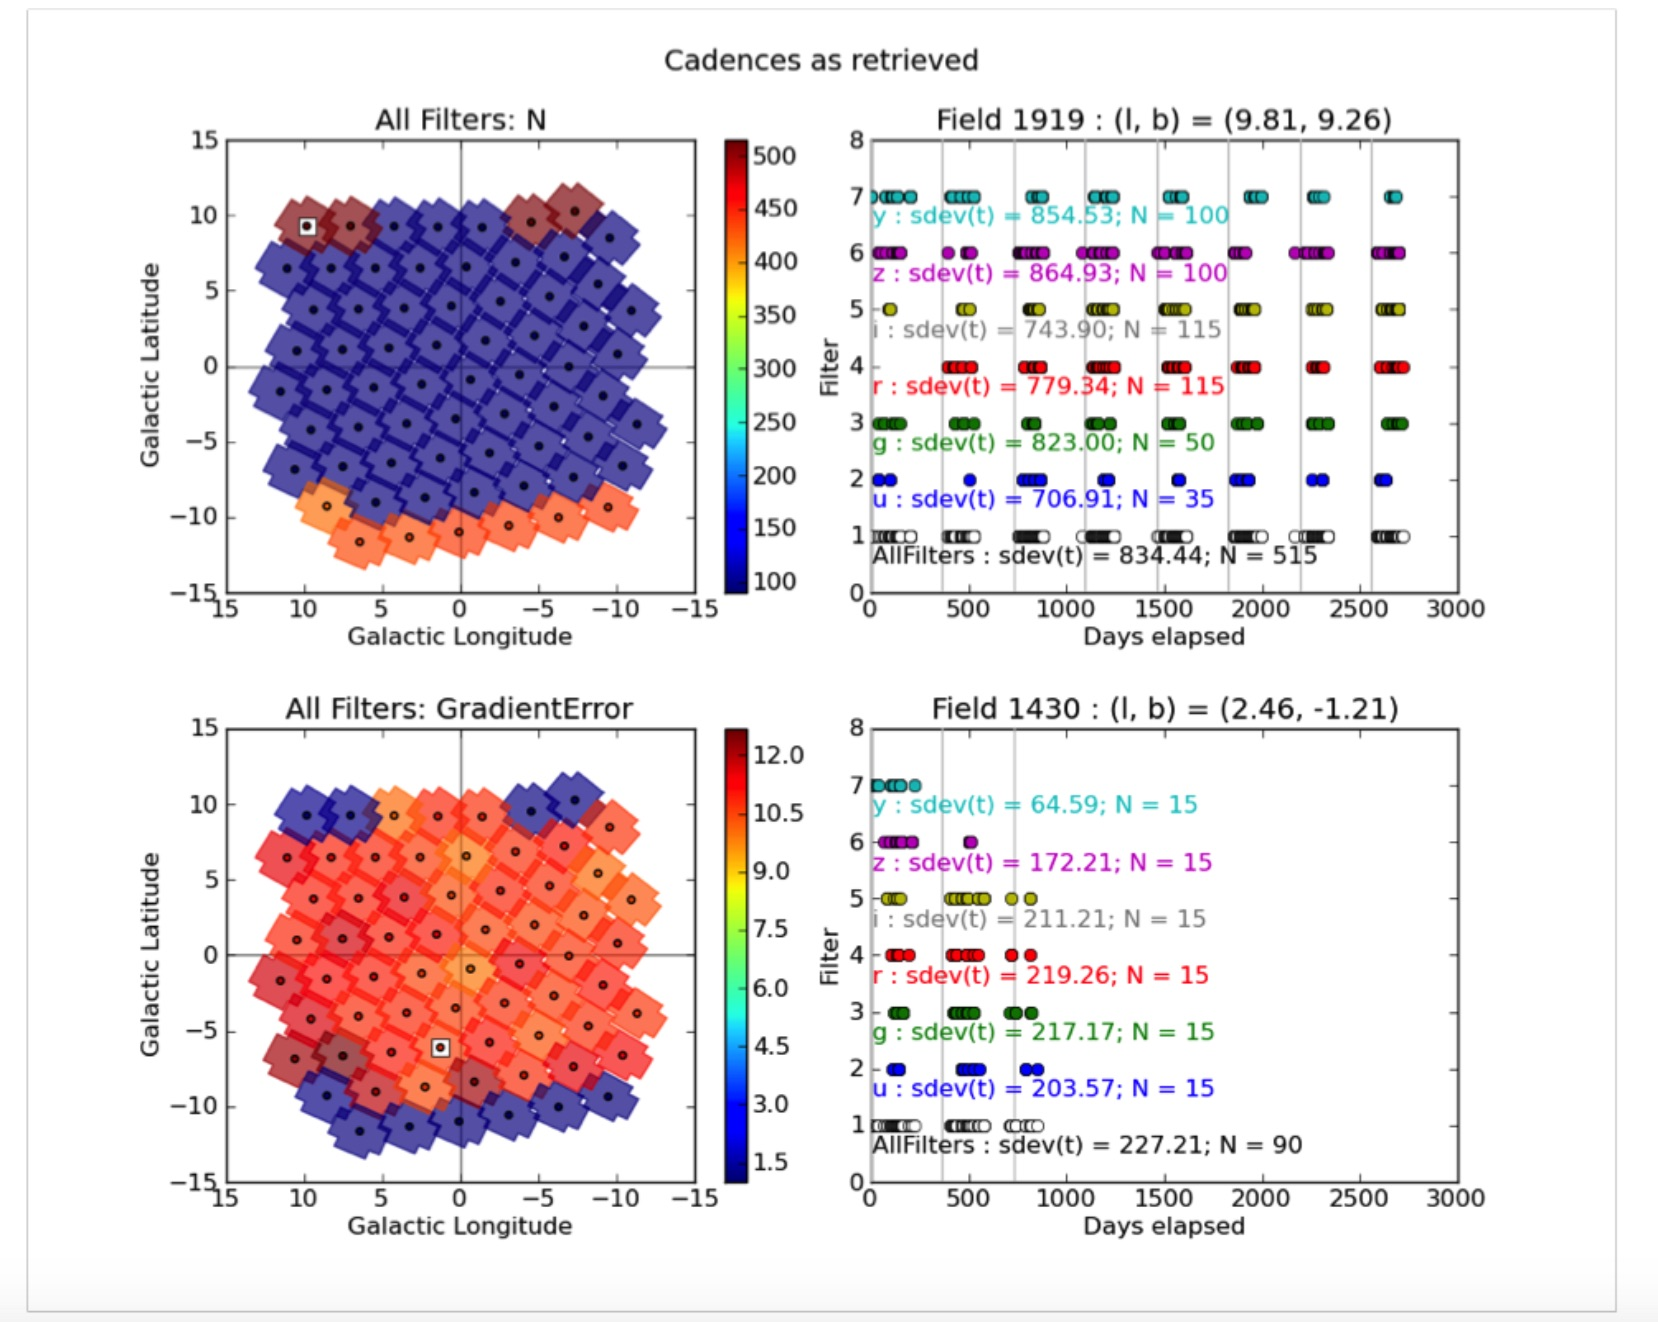
\includegraphics[width=1.0\textwidth]{bulge_fig2a.jpeg}
    \caption{\label{fig:bulge2a}
Figure 2a: This figure shows a basic example of the kind of strategy assessment that could be performed to optimize observations. OpSim was queried for all regions close to the galactic center (-15 < l < 15 degrees) using OpSim as of June 5th 2012, and the dates of all retrieved observations were used to estimate the impact of proper motion measurement due to time allocation and the concentration of observations under the retrieved strategy. Top-left: Map of fields in galactic coordinates, color-coded by the total number of observations per field. 
Bottom-left: Map of fields, this time color coded by the formal error on proper motion based on the samplings retrieved from OpSim. Top-right and Bottom-right show time-series for the samplings for example fields (top = baseline survey, bottom = example bulge field) under the OpSim strategy at the time. All else being equal, the proper motion precision for the Bulge strategy at the time is a factor ~8 worse than the baseline survey just by virtue of the lower time allocation and its concentration, but there are obvious steps that could be taken to improve matters (such as spreading the same observations over the full time baseline of the survey). }
\end{figure}

\begin{figure}[h]
    \centering
    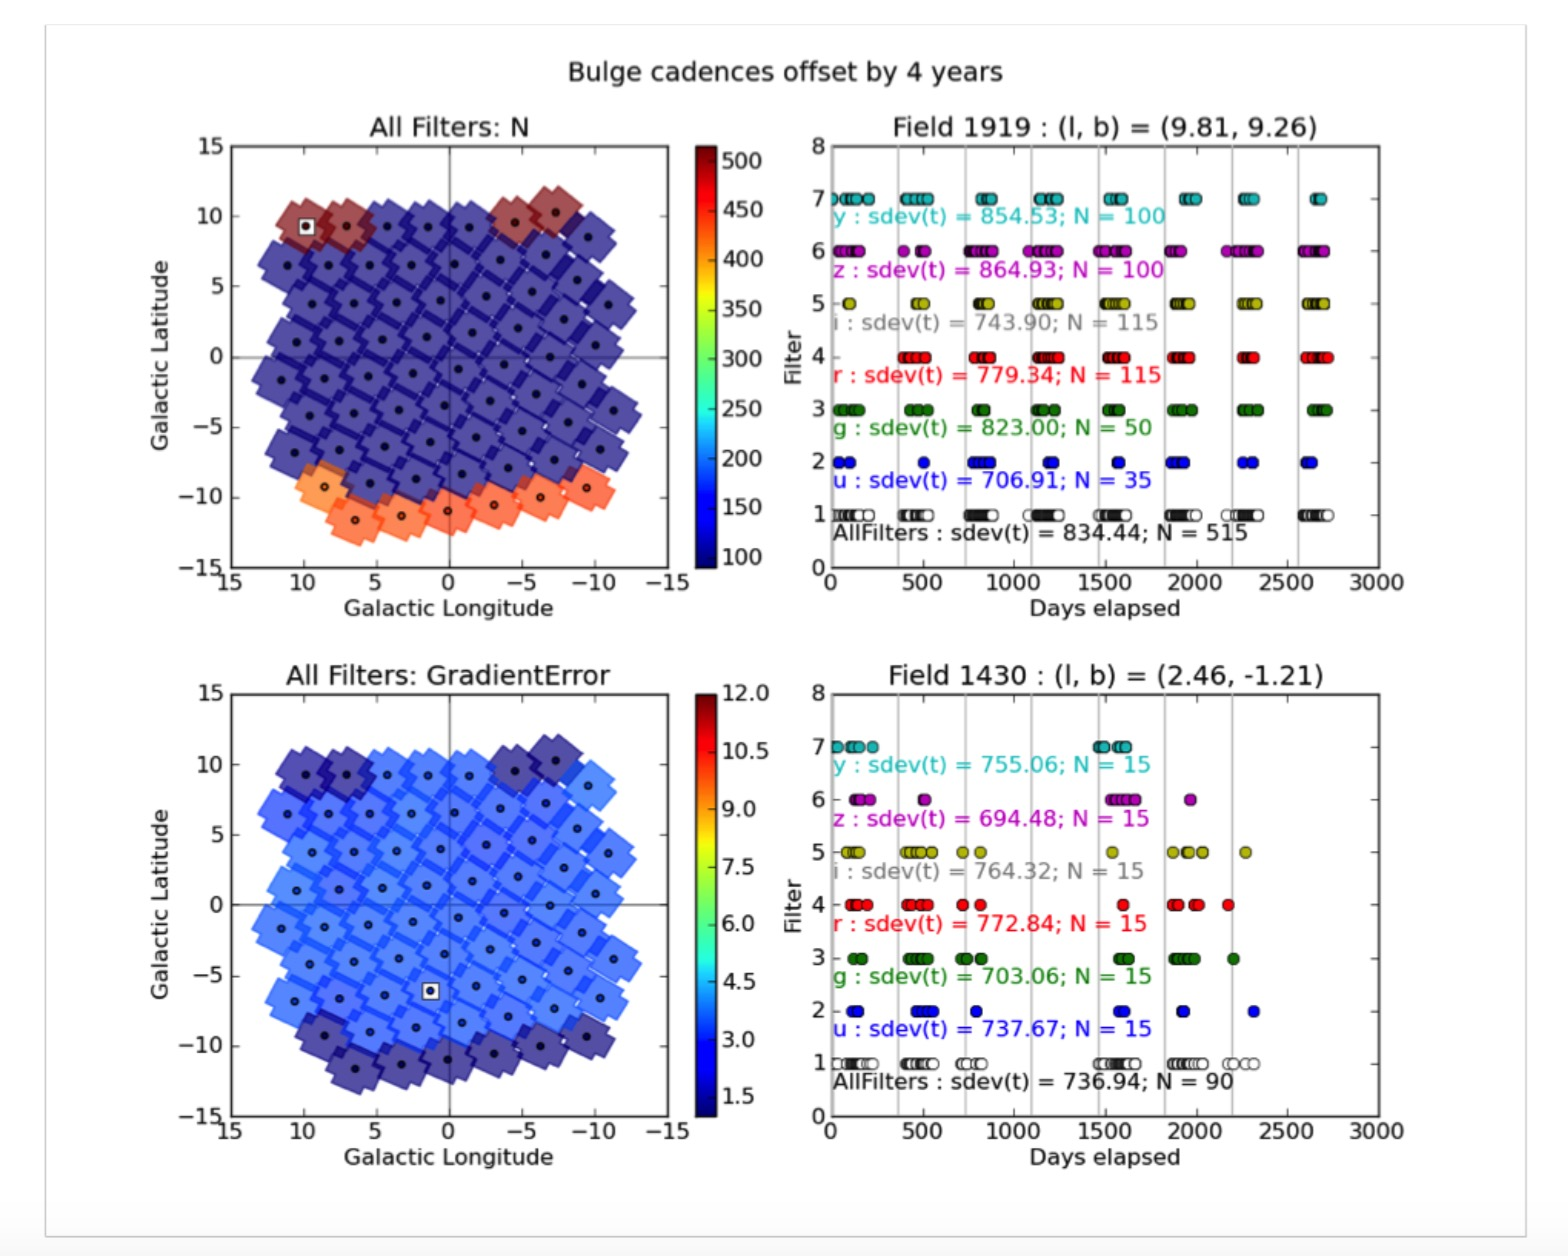
\includegraphics[width=1.0\textwidth]{bulge_fig2b.jpeg}
    \caption{\label{fig:bulge2b}
Figure 2b: As Figure 2a, this time with the original Bulge allocation spread along the same time interval as the baseline survey (note the total number of exposures for the Bulge is the same as for Figure 2a). The formal gradient error has already been reduced significantly, to a factor ~2-3 over the baseline survey. }
\end{figure}



\subsection{Appendix}
more detail about LSST Bulge science goals: To keep the focus of the Phase I document on technical investigations to be performed, much of the detail on the science goals in v0.2 has been moved here. Goals: 
i. Detailed balance of populations as traced by morphology, chemistry, kinematics and distance: 
\begin{itemize}
\item{Morphology: Uniform, accurate positions and magnitudes across sufficiently wide field to characterize 
X-shaped structure. Depth: at least 2 magnitudes below the red clump giants, and ideally down to the 
Main Sequence Turn-off (MSTO). }
\item{Chemistry: Multi-color photometry, with uniformly calibrated photometric zeropoint in each region and 
filter. Depth as per Morphology. Cross-match with NIR catalogs (e.g. 2MASS, particularly VVV) to account 
for interstellar absorption. }
\item{Kinematics, particularly membership probabilities: Tracer stars (e.g. the Red clump giants) may overlap 
significantly with existing and planned spectroscopic catalogs. However, proper motions from LSST itself should allow all stars to be assigned membership probabilities. Requires proper motion precision better than 1 mas / yr, and ideally better than 0.5 mas/yr. }
\item{Distance: Photometric variability will allow standard candles (including but not limited to RR Lyraes, eclipsing binaries) to trace the populations along line-of-sight distance. Requires monitoring cadence sufficient to characterize these tracers. }
\item{Bulge, Thick Disk, inner halo, and Sgr Dwarf: A uniform multiband survey with high astrometric quality that spans the entire inner Galaxy will offer the quantitative means to define how the bulge is related to the inner disk and halo, and to settle whether any “classical” spheroidal-like bulge is separable from the bar. The complexity of the Sgr dwarf populations can be separated from the generally much closer Galactic populations. }
\end{itemize}

ii. The present-day mass distribution of the inner Milky Way (MW), as traced by the Bulge star motions: 
\begin{itemize}
\item{Proper motions: Produce a catalog of proper motions accurate to <1 mas/yr (ideally <0.5 mas/yr) for all 
objects down to the MSTO. Use the wide-field, multi-sight-line nature of this catalog to test models of bulge formation and evolution. E.g. what size of "classical-bulge" population is consistent with the observed velocity dispersion as a function of position and depth? Are the putative kinematic substructures (e.g. Nidever et al. 2012, see also Howard et al. 2009) real? What is the total mass felt by Bulge stars, as a function of cylindrical coordinates (R, theta, phi)? Requires carefully-designed survey strategy. }
\item{Line-of-sight motions: Merging with existing and planned spectroscopic catalogs 3D measured motions for a massive sample of Bulge stars.}
\end{itemize}

iii. Wide-field examinations of other sub-populations and objects of interest: 
\begin{itemize}
\item{Tidal streams and kinematic substructures that pass through the inner MW: With such a wide-field catalog, 
LSST should provide important tracer information for merger remnants and other discrete features in 
phase-space.}
\item{How many Globular Clusters (GCs) exist in the inner MW? VVV is already uncovering more GCs in the inner 
MW, what scientific investigations will LSST enable for these objects? }
\item{
Hypervelocity stars: Observe rare, fast-moving objects ejected from the very inner MW, and use them to 
constrain stellar formation and ejection processes near Sgr A*. }
\item{Is there a “nuclear” population? }
\end{itemize}



\section{Roadmap for Star Clusters Subgroup}

Kevin Covey, Jay Strader, Jason Kalirai, \& Doug Geisler for the subgroup 

\subsection{A short summary of LSST science related to star clusters }

Star clusters are a critical component of many of the science goals listed in the LSST Science Book (Ivezic et al. 2010). They offer unique environments where stars with a range of masses but similar ages and chemical compositions can be found. One class of studies aims to leverage these relatively simple stellar populations to understand the dependence of the stellar mass function and stellar evolution on metallicity and age (e.g., Sec. 6.5-6.6, 6.9-6.11; LSST Sci. Book). Their known properties and distances also motivate calibration work on many kinds of variable stars and transients (e.g., Sec 8.9; LSST Sci. Book). 

A separate class of studies is focused on using star clusters to trace the star formation history, chemical evolution, and galactic structure of the Milky Way, nearby galaxies (including the Magellanic Clouds), and even more distant galaxies extending beyond the Local Volume (e.g., Sec. 6.2-6.3, 6.6, 7.2, 7.3, 7.8, 7.10, 7.11; LSST Sci Book). 

\subsection{Critical technical elements for LSST star cluster science }

The unique advantage of LSST for studies of star clusters is the promise of deep, accurate, and homo- geneous multi-band photometry and astrometry for the entire southern sky. This directly enables both (i) an enormous sample of clusters and (ii) spatially complete data for each cluster, neither of which are generally possible in current datasets. 

This promise can only be realized if LSST delivers photometric and astrometric measurements that are uniform, or at least well-behaved, over the wide range of crowding conditions and variable foregrounds and backgrounds that can occur within a single cluster and across different Galactic components. 

Specifically, we identify the following critical technical elements as most relevant to star cluster science with LSST: 
\begin{itemize}
\item The impact of source crowding and homogeneous backgrounds on the precision and depth of LSST photometry and astrometry. 
\item The performance of LSST’s deblending and multi-epoch source association algorithms as a function of seeing and in crowded or nebulous fields. 
\end{itemize}

\subsection{Near-term investigations to retire risk for LSST star cluster science }

Over the next year, the core members of the Star Cluster Working Group will use simulated LSST data products and precursor datasets to test the expected performance of LSST. Specifically, we plan to: 
\begin{enumerate}
\item{Use the ImSim pipeline to generate synthetic LSST images of crowded fields. Use these to establish the quality of star cluster color-magnitude diagrams—and their utility for testing specific aspects of stellar evolution models—using LSST’s photometry and astrometry. Image morphology statistics will also be used to test star–galaxy separation. (J. Kalirai) }
\item{Obtain the best existing examples of overlapping 
ultra-deep ground-based starcluster photometry with HST images 
(e.g., NGC 5466; Beccari et al. 2013), using the “ground truth” provided by the HST catalogs to empirically assess the expected photometric uncertainties and incompleteness in LSST data. (J. Kalirai) }
\item{Calculate the proper motions uncertainties—both absolute and internal—that LSST will be able to return for typical Galactic star clusters, using both 10-year LSST baselines and longer HST to LSST baselines. These metrics will be compared to Gaia’s expected performance as a function of magnitude and crowding to delineate the opportunity space for LSST in this area. (J. Strader) }
\item{Acquire new, wide-field multi-epoch ugriz photometry of dense and nebulous clusters in the Galactic plane. Process these images with the LSSTstack to quantify photometric precision as a function of local background and assess the fidelity of source association among the epochs. (K. Covey) }
\end{enumerate}

The primary person responsible for each task is listed above, but we expect that much of the effort will be collaborative both within the subgroup and with members of other relevant subgroups. 





\section{Notes towards a roadmap for the Galactic Structure and ISM sub-group}

We have identified three major topics that came out of discussions among the Galactic Structure and ISM subgroup members. We present a number of specific questions that our subgroup would like addressed by the larger collaboration and/or project as well as some specific projects/goals that our subgroup plans to address over the next year. 

\subsection{Crowded field photometry}

Technical overview: The stated limit from the project for the LSST processing is 200 stars/arcmin$^2$,
or 0.056 stars/arcsec$^2$. 
Given that the median seeing at Cerro Pachon is 0.7 arcsec FWHM, the effective beam size is i
$\pi$ * (0.7/2.35)$^2$ = 0.28 arcsec$^2$. 

Thus the proposed LSST limit is at 64 beams / source, or at $\sim$half the 30 beams / source confusion limit.
 
Implications for Galactic Structure science: 
\begin{enumerate}
\item In what fields do we hit the proposed limit and the confusion limit as a function of band and Galactic coordinates for a single 15-second exposure? Action: We propose to organize an effort to estimate these values based on empirical data rather than simulated data, the latter of which are based on extrapolations. 
\item What are the Galactic Structure science goals that require the fields having densities greater than
 200 stars/arcmin$^2$ but less than the confusion limit? Action: This depends on how many fields are above that and where they are. 
\item What model does ImSim use to create the Galactic Disk and Bulge stellar populations? Has this been tested at, e.g. low Galactic latitudes? Action: We can actually correct the ImSim using results from (1). 
\end{enumerate}

\subsection{Astrometry [feedback from the DAWG]}

The following questions came from members of the sub-group – we summarize the most important aspects of them in hopes of geting answers/feedback from the project: 
\begin{enumerate}
\item Will the project assume responsibility for crowded field photometry and astrometry software? 
\item Regardless of the project's support for crowded fields, should the science collaborations investigate alternative algorithms? 
\item Should there be (or is there already) an ensemble of ImSims upon which the science collaboration members can try their algorithm and then compare their results against the “truth” (inputs to ImSim)? 
\item What are the mechanisms for ensuring that certain features/capabilities are part of ImSim, the photometric pipeline or other project-wide software/tools? 
\end{enumerate}

Specifically, one of our members (D. Monet) reports that astrometric studies show that the ImSim does not
mimic real data and that the astrometric errors grows as a function of separation. 
Also, the generation of 20 simulations that differ by only the seed used for the random number generator
 results in changes in the sky background of a factor of 30. 
They go from 0.1 to 3 times the value listed in the SRD. 

\subsection{Y4-band}
 There was some discussion in our sub-group about the performance of the y-band filter. 
Specifically, some users were concerned about the ability to calibrate out water vapor. 
Some of the specific cases where this may be important have clear overlaps with the low-mass star 
(and other) sub-groups but we summarize some of the discussion and specific questions below. 

The main science cases that came up were motivated by the need for creating a color calibration of the 
M dwarf photometric metallicity scale and the identification of cool subdwarfs with the y-filter in 
combination with griz. These calibrations could directly lead to examining the distribution and scale 
height of M dwarfs as a function of metallicity and potentially probe the contribution from 
extragalactic streams and/or other halo object. 

Potential Issues with the y-band filter: 
\begin{enumerate}
\item{Water vapor – an unresolved problem in the y4-filter is the highly time variable effect of water vapor 
and whether it can be removed – and if so, at what precision. 

Action: Members of our sub-group were curious if there exist time series spectra that would allow our sub group (or in tandem with others) to assess how easily the y4 band can be calibrated and what the empirical solution is to this concern. If these data don't exist, are there plans/ability to acquire these data? 
If the data do exist then one of our sub-group’s action items will be to investigate the calibration and precision of the y-band filter (see (2)). }

\item{Metallicity calibration and identification of low-mass subdwarfs – our sub-group is committed to 
assessing how the y-filter (irrespective of (1)) will affect identifying and classifying the very 
metal poor halo M dwarfs accurately (disentangling temperature and abundance effects) as well as creating a useable photometric metallicity scale. The current SDSS gri color-color diagrams show significant overlap among metallicity classes of low-mass stars. And while most of the SDSS objects have spectroscopy, almost all of the extremely faint LSST stars will not. 

Action: Our sub-group has identified a number of questions that will lead some of our effort of the next year. These include (but are not limited to): Is there any way to increase the photometric accuracy in the classification and identification of metal-poor, low-mass stars? What are the quantitative limits to our precision with the current LSST setup (including the y4 filter)? Are there other observations that we can persue that might help answer these questions? Members of our sub-group have done some modeling using existing spectra. However, there are limited data for the coolest, lowest mass, and most extreme subdwarfs. These extreme stars are the ones near the hydrogen-burning limit that will ultimately tell us about the bottom of the mass function in the early history of the Galaxy. 
Therefore, one additional action item is to acquire additional low-mass subdwarfs to continue modeling LSST photometric products. }
\end{enumerate}


\section{LSST Near Field Cosmology Roadmap}

The LSST Near Field Cosmology subgroup focuses on using stellar substructure throughout the Milky Way
 and Local Volume as a probe of the underlying CDM cosmology. 
This includes searches for dwarf galaxies, tidal streams and other coherent features in 
phase space using the properties of individual stars. 
Examples include searches for ultra-faint galaxies based on overdensity of main sequence stars, 
searches for substructure using RR Lyrae variables, or searches for moving stellar groups using proper motions. 

Searches for Milky Way substructure will allow critical new constraints in several areas. 
A more complete census and map of the distribution of satellites around the Milky Way sheds 
light both on the formation of satellite systems and the nature of dark matter halos that are 
able to host such low-mass galaxies.
 Finding tidal debris beyond 100kpc and out to the virial radius of the Milky Way will open a 
window on the more recent accretion history of the Galaxy, as well as the accretion of objects 
on more radial orbits in particular. 
Debris in the outer Galaxy also promises a powerful new probe of the mass 
distribution around the Milky Way in regions of a dark matter halo that have been largely 
unexplored for any galaxy in the Universe. 


\subsection{Overview of LSST NFC Science Goals}
\begin{itemize}
\item Mapping Milky Way substructure, including dwarf galaxies and stellar streams using main 
sequence stars out to $\sim$300kpc 
\item Map of Milky Way substructure using more luminous tracers (BHB, RRL) out to 800 kpc 
\item Search for substructure in tangential velocity field out to 25 kpc 
(60 km s$^-1$ precision). 
\end{itemize}

\subsection{Scientific and Technical Issues}

We discuss below issues that go beyond the LSST design specifications. 
\begin{enumerate}
\item{StarGalaxy Separation: For apparent magnitudes beyond $r\sim22$, the number of unresolved
 galaxies relative to stars rises dramatically. StarGalaxy separation is critical and 
improvements in StarGalaxy separation will likely have 
the most significant influence on the degree to which the above
 science goals are achieved. 

StarGalaxy separation will be done using both color and morphological criteria. 
There is general consensus that these two type of criteria remain separate in the 
LSST catalogs, allowing users to combine them in different ways for different science goals. 
combined for specific science goals. There is a desire to see as many measures relevant to
StarGalaxy separation as possible. Preferably as a probability, or some index like ($\chi^2, \nu$)
 that is transformable to probability. }

\item{AllSky Query Capability: Search for Milky Way substructure, particularly tidal streams, 
may be one of the few sciences cases that requires full survey data access and cannot be 
accomplished on smaller data chunks. This is unlikely to be possible in SQL on LSST servers. 
An SDSSLike Casjobs interface is both necessary and sufficient for this. }

\item{Variable Stars: The NFC group is primarily interested in RR Lyrae, but additional variable 
stars include W UMa stars, $\delta$Scuti, Miras and Cepheids are of interest. 
There was general agreement that current LSST cadance is sufficient for these searches.
 Important flags to search for variable stars include the Stetson J, K, and L indices, as well as the
 median magnitude, skewness, kurtosis, von Neumann index, and linear fits to magnitudes vs. time.}

\item{Flags for diffraction spikes, ghosts, etc: 
Searches for substructure depend critically on photometric uniformity. 
Need to have a catalog flag indicating the degree to which a source may be a 
product of (or affected by) diffraction spikes or ghosts. 
It is important that these flags are provide for each data epoch.}

\item{Proper Motion Flags: 
Both straightline measurements as well as with parallax folded in, with a 
$\chi^2$ for each. 
This would be good both to identify nearby stars as well as improve 
reliability of the proper motions of distant stars with too many fitting parameters. }

\item{Completeness Estimates: Many NFC science goals will require estimates of the sample
 completenesses as a function of magnitude for point sources in each color, at every position on the sky.
 This involves artificial star tests over an appropriate range of seeing, crowding, 
and for the appropriate number of exposures that go into each data release's average 
photometry. This will be particularly true for coadded data products.}
\end{enumerate}


\section{Towards a Roadmap for LSST Magellanic Clouds Science}
Knut Olsen, with direct contributions from Nitya Kallivayalil, Beth Willman, Doug  Geisler, and Ben Williams  

\subsection{Introduction} 
The LMC and SMC are the nearest large galaxies to the Milky Way and represent  fundamental testbeds for investigations related to many stellar astrophysical topics,  from studying the star formation process, to the physics of variable star populations,  to the physics of galaxy interactions, and to calibrating the cosmological distance  scale.    

The Clouds are some of the bestGstudied galaxies in the Universe, yet nevertheless  consistently have the power to surprise.  A recent surprise is that the Clouds, which  have long been thought of as closely bound satellites of the Milky Way, appear to be  on first infall, or at most have made a small number of close passages, based on  proper motion measurements (Kallivayalil et al. 2006a,b; Besla et al. 2007, Piatek et  al. 2008, Kallivayalil et al. 2013).  We have also seen evidence that the LMC has  accreted a significant mass in stars from the SMC (Olsen et al. 2011), which may  indicate that the LMC and SMC collided directly with each other ~100 Myr ago  (Besla et al. 2012), a discovery that relied on the proper motion work.  The HI tidal  streamers that connect the LMC to the SMC and Magellanic Stream are kinematically  linked to the accreted SMC stars, and thus may have formed in this collision; the  streamers converge on the location of 30 Doradus in the LMC (Nidever et al. 2008),  indicating that 30 Doradus may be an interactionGinduced star formation event.   Moreover, the stellar debris left behind by the SMC could naturally explain the  microlensing event rate (Besla et al. 2013) seen towards the LMC by e.g. MACHO and  OGLE.  

The Magellanic Clouds are also now known to extend to much larger radius than  known before, through several pencilGbeam studies.  Majewski et al. (2009) found  spectroscopicallyGconfirmed KGgiant LMC stars at large distances (R $\sim$ 22 or 19 kpc),  while Saha et al. (2010) found that the LMC exponential disk extends past 12 disk  scale lengths.  In the SMC, Nidever et al. (2011) traced K giants to $\sim$11, with  possible evidence for a stellar halo.  These studies are based on exploration of 1  of the relevant area of sky.  There is thus a vast area that remains to be explored for  hidden Magellanic Clouds structure, with implications both for understanding the  history of the Clouds and the formation of the Galactic halo.   

There are many other recent exciting discoveries in the Magellanic Clouds that have  not been mentioned here.  The point of mentioning the few above is to demonstrate  that 1) in the Clouds, astrophysical problems are often connected across broad areas  of study, 2) Magellanic Cloud populations cover a very large area of sky, and 3)  highly precise measurements, such as produced by the work on LMC and SMC  proper motions, have the power to fundamentally alter accepted understanding.  

\subsection{LSST:relevant Magellanic Cloud Science Objectives}
 Magellanic Clouds science potentially covers a very broad range of topics.  Some of  the topics that the MC working group suggested of being of greatest interest are:  
\begin{enumerate}
\item{Mapping the Magellanic periphery.  Magellanic Cloud populations are now  known to extend out to ~20 degrees from the parent galaxies.  Whether  these populations are related to stellar halos, extended disks, or tidal debris  is not known.  The HI Magellanic Stream extends over 200 degrees of sky  (Nidever et al. 2010).  LSST will excel at finding stellar populations down to  very low effective surface brightness through deep photometry of individual  stars.  It will also provide a vast sample of RR Lyrae to trace potential  structures in three dimensions.  }
\item{Proper motions and internal motions.  The most precise proper motions in  the Clouds so far are those based on HST observations of narrow fields  centered on background QSOs (Kallivayalil et al. 2006).  LSST has the  potential to deliver precise proper motions over large swaths of the Clouds.   Given the complexity in the internal kinematics, these would be a boon for  piecing together the effects of the LMC and SMC recent interaction history.   As a demonstration of what is potentially possible, CasettiGDinescu et al.  (2012) found a significant proper motion difference between the  spectroscopically identified accreted SMC stars in the LMC and the general  LMC background, using groundGbased measurements.  }

\item{The star formation and chemical abundance history of the Magellanic Clouds.   Linking detailed knowledge of these to detailed knowledge of the interaction  history of the Clouds will be a big step forward in understanding what has  driven the evolution of the Clouds’ stellar populations.  }

\item{ Stellar variables.  The Magellanic Clouds contain the full array of known  variable stars, with the big advantage that their distances are well  constrained.  They also give important insight into variable star physics  through their low metallicities compared to the Milky Way.  Important  variable star classes are regular variables such as RR Lyrae, irregular  variables for which the Clouds provide complete statistical samples of events  such as flares, variables which are discovered at wavelengths other than  optical, such as xGray binaries, and stars which experience eclipses by other  stars or, potentially, planets.  }

\item{Star clusters.  The Magellanic Clouds are thought to contain thousands of star  clusters, only a fraction of which have been discovered and cataloged.  Star  clusters are very useful as precise markers in age and metallicity in the  history of star formation in galaxies, and critical for understanding questions  related star cluster dissolution and star formation mode.  LSST has the  potential to provide a complete catalog of Magellanic Cloud clusters to great  depth, including clusters at large radius from the parent galaxies.  }
\end{enumerate}

\subsection{Scientific and technical issues}
 The first big scientific issue is to identify those science cases that are uniquely  enabled by LSST.  In the case of the Magellanic Clouds, the existence of other largeG 
scale optical surveys such as the Magellanic Clouds Photometric Survey (Zaritsky et  al. 2000), DENIS, and the Dark Energy Survey, as well as the existence of wideGfield  cameras such as DECam, can give the impression that the science cases outlined can  be done by other means.  While it is certainly true that past and current surveys are  working on the problems above, LSST has the potential to open qualitatively new  discovery spaces through:  
\begin{enumerate}
\item{ Deep, multiepoch coverage of nearly the entire southern sky.  We have  
already shown that the search for Magellanic Cloud populations is one that  potentially covers thousands of square degrees.  While DES and the DECam  survey SMASH (Nidever et al. 2013) will be potential bonanzas for the study  of the Magellanic periphery, they probe only to g~24, the single'epoch depth  of LSST, and have limited time information.  LSST stacked photometry will go  several magnitudes deeper, yielding the potential to discover structure with  extremely faint equivalent surface brightness, and allow for the use of  variable stars as three dimensional probes of structure.  }

\item{Precise proper motions.  Much of our recent advance in revealing the  complexity of the Magellanic Cloud interaction history stems from the factor  of 10 improvement in proper motion that the HSTGbased work provided.  If  enough attention is given to the Clouds in the LSST cadence, LSST has the  potential to reveal the internal motions of the Clouds in unprecedented detail.  }

\item{Precise photometry.  All of the work described above depends on  photometric measurements.  Given the scale of typical PIGled projects and  calibration efforts, it is rare for projects to achieve <2  photometric  accuracy in the absolute sense.  The LSST science requirement is to deliver  1  absolute photometric accuracy in single images, with a stretch goal of  0.5 .  If these numbers can be achieved for the Clouds, and in particular  improved upon by averaging multiple measurements, metallicities based on  photometry, ages from comparison to isochrones, and reddening  measurements all stand to improve by large amounts.  As demonstrated by  the phenomenal results from Kepler, the realm of high photometric accuracy  has the potential to deliver many surprises.  }
\end{enumerate}

  Given the discovery spaces that will make LSST unique for Magellanic Clouds  science, there are a number of technical issues that need to be addressed as part of a  roadmap for the Magellanic Clouds:  
\begin{enumerate}
\item{What cadence is needed for full Magellanic Clouds coverage to achieve the  desired gains in proper motion and photometric accuracy?  The main bodies  of the Clouds, in the current baseline, are not part of the WideGFastGDeep  survey, but are covered at reduced frequency.  
\begin{enumerate}
\item{To evaluate the astrometric needs, we can quantify what HST/GAIA  can do per single star, and what requirements that imposes on LSST  observing in the MCs.  Dave Monet has been doing a lot of work within  the context of the DAWG to come up with metrics that best define  astrometry errors. Nitya summarizes from Monet: we want to (a) give  
specific examples of good and bad parallax cadences, and also (b)  develop metrics that can predict good and bad cadences so we can  optimize. So far, the former has shown that there is a factor of 2  difference in recovered errors based on cadences that otherwise take  the same amount of telescope time, and also as far as (b) goes, we  don't have a good metric so far, and all the various metrics one could  come up with seem to be correlated.  }

\item{To evaluate the level of photometric accuracy that we achieve in the  Clouds and the resulting cadence requirement, we can use the DECam  observations that are getting underway to begin answering this  question.  }
\end{enumerate}
}
\item{What limit on the photometric and astrometric accuracy is crowding going to  impose on us?  
\begin{enumerate}
\item{Past observations and the ongoing DECam surveys can help answer  the question of the fundamental limit imposed by crowding.  }

\item{How crowded images will get handled by LSST DM is a separate  question, and will require interaction with the DM Stack with  comparisons to crowded field photometric packages such as  DAOPHOT.  }

\item{A related question is whether there is the potential for a limited set of  excellent seeing observations in the Clouds, and whether that would  adversely impact the global cadence.  }
\end{enumerate}
}
\item{What is the best approach to starGgalaxy separation, particularly important  for studying the Magellanic periphery?  
\begin{enumerate}
\item{The SMASH survey has begun to address this question to the level of  r~24, but the growth in the galaxy luminosity function at faint  magnitudes means that we’ll probably need a dedicated effort to test  this to the depths that LSST will achieve.  }
\end{enumerate}
}
\item How do we accommodate the need for artificial star tests?  
\item{What other datasets need to be crossGmatched against the LSST catalog for  
the project to succeed?  a. We can begin constructing a list pretty easily.  }
\item{Are there particular projects that would be compelling/easy to do early in  the survey, perhaps during commissioning?  }
\item{What are the typical database queries and data services that we will be  using?   
a. This will need to be explored. There are efforts underway to provide a  testbed for potential services that would be useful to interact with  here.  }
\end{enumerate}


\section{LSST Solar Neighborhood Collaboration Roadmap Planning Document }

Adam Burgasser, John Gizis, Todd Henry, Sebastien Lepine, Michael Liu, Keivan Stassun 



\subsection{Purpose of this Document }
\begin{itemize}
\item{Identify 
the technical and scientific challenges for LSST in studying low mass stars and  the solar neighborhood }
\item{Identify 
tasks for collaboration members that can overcome these challenges on a  timescale of a few years. }
\item{Organize 
collaboration members to perform assigned tasks before data delivery }
\end{itemize}


\subsection{History }

\begin{itemize}
\item 22 October 2013 (AJB): Version 1 released to working group 
\item 1 November 2013 (AJB): comments integrated and sent to leads 
\item 2 January 2013 (AJB): comments from WIllman 
\item 14 August 2014 (MCL): cleanup of edits 
\end{itemize}

\subsection{Introductory Material}

\subsubsection{Key target populations:}
\begin{itemize}
\item{Solar 
neighborhood: classically d $<$ 10-25 pc, extend to $\sim$100 pc in LSST era}
\item{Young 
stars: clusters, moving groups \& associations }
\item{Old 
stars: subdwarfs, thick disk and halo objects, globular clusters (??) }
\item{Brown 
dwarfs: $<$0.07 Msun, including free-floating planets }
\item{White 
dwarfs (and other remnants?) }
\item{Binaries 
and higher order multiples: q $>$ 0.1, resolved and unresolved}
\item{Low 
mass companions: q $<$ 0.1, resolved and unresolved }
\end{itemize}

\subsubsection{Definitions \& Acronyms used in the text}
Mass scales: 
\begin{itemize}
\item{$>$ 
2 Msun = “massive” }
0.5-2 
\item{
Msun = “solar type” }
\item{0.1-0.5 
Msun = “low mass” (LM) }
\item{$<$ 
0.1 = “very low mass” (VLM) }
\item{$<$ 
0.07 Msun = “brown dwarf” (BD) }
\item{$<$ 
0.013 Msun = “planetary-mass object” (PMO) }
\end{itemize}


CPM = common proper motion  DBMM = deuterium burning minimum mass, nominally 0.013 Msun for solar Z  GC = globular cluster  HBMM = hydrogen burning minimum mass, nominally 0.07 Msun for solar Z  LBMM = lithium burning minimum mass, nominally 0.06 Msun for solar Z 
[M/H] = metallicity 
MF = mass function  MG = moving group  MS = main sequence star  NIR = near infrared  PM = proper motion  PMS = pre-main sequence star  RPM = reduced proper motion  RV = radial velocity 
 SED = spectral energy distribution  SpT = spectral type  ToO = target of opportunity  WD = white dwarf  YA = young association  YMG = young ($<$100 Myr) moving group 

\subsection{Roadmap Plan }
\begin{itemize}
\item{Phase 
1 (deadline: 1 Nov 2013): Highlight technical/scientific challenges that must be  worked on to conduct our science with LSST. }
\item{Phase 
2 (deadline: TBD): Develop a strawman path towards overcoming those  challenges before LSST data start flowing. }
\item{ Phase 
3 (deadline: TBD): raise interesting precursor science that can be done by  you/can get grant support now. }
\end{itemize}


\subsection{Identified inputs required for planning (priorities TBD)}
\begin{itemize}
\item{precise 
LSST filter definitions }
\item{photometric 
sensitivity per band for single and deep pointing }
\item{astrometric 
performance (proper motion \& parallax) per band as a function of 
brightness, spectral type, \# of epochs, time baseline and sky location (see preliminary 
results from DAWG = Differential Astrometry Working Group) }
\item{LSST 
imaging cadence(s) }
\item{LSST 
PSF shape model (including saturation) }
\item{galactic 
model }
\item{ spectroscopic 
followup resources }
\item{theoretical 
atmospheric models of LMs/VLMs/BDs as a function of {Teff, log g, [M/H], 
clouds, circulation} that span LSST bands }
\item{empirical 
templates of sources (MLTY standards, subdwarfs and young dwarfs) }
\item{evolutionary 
models and forward modeling samples for BD population }
\item{flare 
emission model to determine LSST response/sensitivity to LM flares }
\item{cloud 
spot model to determine LSST response/sensitivity to BD weather patterns }
\item{An 
(updateable) list of currently nearby LMs/VLMs/BDs (ra, dec, spt, distance, predicted 
LSST mags, age/cluster, etc) }
\item{Quantification 
of completeness as a function of SpT and distance }
\end{itemize}

\subsection{Primary science investigations: Objectives, issues and tasks}



\subsubsection{Volume-complete (astrometric) sample of extended solar neighborhood }

definition: all sources for which parallax measurements can be made with LSST  

interested collaborators: 
Adam Burgasser,
John Gizis,
Todd 
Henry,
Michael 
Liu,
Keivan 
Stassun,
Sebastien 
Lepine.

interface with other collaborations: 
Galactic Structure and ISM: 

objectives:
\begin{itemize}
\item distance-limited sample of solar neighborhood (to be defined) 
\item 6D phase space determination (XYZUVW) 
\item LM/VLM/BD MF determination 
\item Full physical, atmospheric, multiplicity characterization of complete sample  
\item map evolution of ultracool objects through the M/L, L/T, and T/Y transitions. 
\end{itemize}


issues: 
\begin{itemize}
\item number of epochs and cadence required to distinguish proper motion and parallax 
\item overlap with GAIA (minimal/non-existent for L/T/Y dwarfs) 
\item astrometric calibration and astrometric uncertainties 
\item distance limit for completeness 
\item brightness limit for completeness (e.g., astrometric accuracy vs. brightness) 
\item detection of/contamination by astrometric binaries and unresolved binaries 
\item followup spectroscopy: science goals \& data needs (sample size, resolution, etc.) 
\item RV measurements 
\item kinematics (statistical) ages? 
\item handling crowding along Galactic plane (e.g. image differencing, pixel-level modeling) 
\end{itemize}

tasks to do: 
\begin{itemize}
\item{need 
a current list of stars (perhaps broken down by SpT) w/in XX pc to assess where the 
big holes in completeness are - both X and SpT regime that we care about will need to  be defined (Todd?), will require some “population synthesis” modeling for BDs (Adam?),  as well as kinematic considerations (Paul Thorman?) }
\item{summarize 
existing compliations from Pan-STARRS solar neighborhood work (Mike) }
\item{model 
astrometric binary contribution/contamination }
\item{comprehensive 
follow-up of sources - RV, high resolution imaging }
\item{examine 
model parameter sensitivity through LSST photometry }
\item{Lists 
of proper motion selected M dwarfs already exist to at least 100 pc. A local  kinematics model (velocity space distribution), combined with luminosity function, will  determine how many stars are missing from the current census as a function of  magnitude, and e.g. what the distance range of GAIA will be for stars of different  magnitudes. This will determine the “sweet spot” (in distance/luminosity) for LSST to  reap the most results. }
\end{itemize}


tasks completed: 

\subsubsection{Deep sample of LM/VLM/BD dwarfs}

definition: sources inaccessible to parallax  

interested collaborators:  

interface with other collaborations: 
Galactic Structure and ISM: 
The Galactic Bulge: 
Near Field Cosmology: 

objectives: 
\begin{itemize}
\item{extremely 
large sample ($10^6$?) for population analysis }
\item{galactic 
stratigraphy - chemical abundances, kinematic “heating”, structural features 
out to XX kpc }
\item{galactic 
scaleheight as a function of mass (constraint on potential and formation 
mechanisms)} 
\item{search 
for thick disk/halo objects }
\end{itemize}

issues: 
\begin{itemize}
\item{spectroscopy 
won’t be viable for whole sample - photometric selection criteria, RPM 
(limits) }
\item{most 
sensitive filter likely to be Y(4): will single-band detections(+astrometry) be useful? }
\item{limit 
to which PM is viable }
\item{metallicity 
characterization through photometry alone }
\end{itemize}

tasks to do: 
\begin{itemize}
\item{simulate 
yield along different sitelines, with variations in scale height, MF, etc. }
\item{calibration 
sample for metallicity effects  tasks completed: }
\end{itemize}


\subsubsection{Ultracold brown dwarfs (late-T and Y dwarfs)} 
definition: BDs cooler than $\sim$1000 K => T5 and later, any distance  

interested collaborators: 
Adam Burgasser, Michael Liu 

interface with other collaborations: 
Galactic 
Structure and ISM: 

objectives: 
\begin{itemize}
\item{detect 
a significant population of T and Y dwarfs for MF determination }
\item{kinematic 
characterization (6D phase space) }
\item{identify 
extreme TY populations (halo, young, cloudy, etc.) }
\item{measure 
how optical SEDs change across K$->$KCl, Na$->$NaCl/Na2S transitions }
\end{itemize}

issues: 
\begin{itemize}
\item{sensitivity 
of LSST filters to cool T and Y dwarfs - detection limits, expected numbers 
assuming an MF }
\item{compare 
expected performance to WISE. 
e.g. LSST will not be competitive in this area, 
at least for discovery of the coolest objects. }
\item{most 
sensitive filter likely to be Y(4): will single-band detections(+astrometry) be useful? }
\item{possible 
to spectroscopically follow these up? (necessary for classification, RV) }
\item{minimal 
information set required to eliminate contaminants (e.g., RPM, color sets, 
necessary filters) }
\end{itemize}

tasks to do: 
\begin{itemize}
\item{examine 
photometric classification and contamination}
\end{itemize}

tasks completed: 


\subsubsection{Halo dwarfs across the substellar limit}

definition: dwarfs with halo kinematics and/or $[M/H] \le -1$  

interested collaborators: 
Pat Boeshaar,  Adam Burgasser, John Gizis,  Michael Liu,
Sebastien Lepine 

interface with other collaborations: 
Galactic 
Structure and ISM: 

objectives: 
\begin{itemize}
\item{Halo 
mass function across substellar limit}
\item{measurement 
of H-burning “age gap” (z-dependent HBMM)}
\item{confirmation 
of BD formation in low metallicity environment}
\item{metallicity 
effects on low mass spectra/photometry }
\item{multiplicity 
of halo LM/VLM/BD dwarfs }
\item{map 
out velocity space distribution }
\item{search 
for substructure in LM halo }
\item{discovery 
of extremely metal poor ($[Fe/H] < -3$) VLM dwarfs }
\item{Pop 
III VLM dwarfs? }
\end{itemize}

issues: 
\begin{itemize}
\item{game 
selection: target max V (anticenter and vertical ring) }
\item{efficient 
and robust selection: RPM, metallicity effects, contaminants}
\item{mapping 
LSST photometry to physical properties - templates? models?}
\item{spectral 
characterization? }
\end{itemize}

tasks to do: 
\begin{itemize}
\item{model 
discovery rate using MF forward modeling + atmosphere models (colors) }
\item{identify 
templates for SED characterization }
\item{estimate 
the local density of halo subdwarfs and their expected magnitude/color 
distribution, based on the existing census. }
\item{Calculate the distance range over which LSST  will be detecting M subdwarfs of different subtypes, what can be expected of their  proper motion distribution, and determine the distance range required to assemble  statistically significant samples of various metallicity classes (i.e. halo sub-populations). }
\end{itemize}

tasks completed: 


\subsubsection{Co-moving populations}

definition: members of well-defined clusters, 
young associations, and moving groups in the  Solar Neighborhood 

interested collaborators: 
Michael Liu, Keivan Stassun, Sebastien Lepine 

interface with other collaborations: 
Star 
Clusters 

objectives: 
\begin{itemize}
\item{complete 
MFs for YAs/MGs in VLM/BD regimes }
]tem{search 
for new YAs/MGs, 
associated with “isolated” stars or as completely new groups. }
\item{identify 
ultracool dwarf benchmarks over a broad range in age ($\sim$1 Myr to $\sim$1 Gyr) }
\item{build 
up sample of ultracool dwarf benchmarks (i.e. with well constrained ages, 
compositions, distances) }
\item{disk/jet/accretion 
properties of young group members (e.g., TWA) }
\end{itemize}


issues: 

\begin{itemize}
\item{
probability 
of cluster membership: CPM, $\pi$/Dest, phot/spec properties, UV/X-ray, 
variability?; are RVs necessary? }
\item{how 
to we obtained activity diagnostics to examine youth? (e.g., Halpha) }
\item{Will 
u photometry be sufficient to characterize UV emission excess? }
\item{disentangling 
multiple memberships (overlapping nearby groups) }
\item{what 
is lowest mass we can probe to in a given group? }
\item{mapping 
observations to physical properties (Teff, logg, masses, ages) }
\item{mass 
sensitivity limit for nearest GCs, older clusters (including age effects) }
\item{The 
young local pop will start to merge with ScoCen - how do we interface with the Star 
Cluster subgroup?}
\end{itemize}

tasks to do: 
\begin{itemize}
\item{ determine 
requirements on RV measurement for cluster association }
\item{
confirm 
and compile properties of nearby YAs/MGs/GCs }
\item{predict 
mass limits for various groups }
item{
characterize 
impact of disk/jet emission/envelope obscuration on LSST (+2MASS 
+WISE?) photometry, map color terms to physical measures}
\end{itemize}

tasks completed: 



\subsubsection{VLM Multiples}

definition: all multiples with a VLM/BD primary, including PMOs  

interested collaborators: 
Adam Burgasser,  Michael Liu

interface with other collaborations  

objectives: 
\begin{itemize}
\item{measure 
the wide separation binary fraction and separation distribution via CPM }
\item{measure 
the small separation binary fraction via astrometric binaries }
\item{detect 
eclipsing binaries; if sufficient number, measure binary fraction at close 
separations }
\item{ use 
these measurements to constrain separation and mass ratio distributions, binary 
fraction all as a function of mass/SpT }
\item{use 
astrometric and transit binaries to determine orbital distributions (eccentricity, 
mass ratio) }
\item{use 
transit binaries to test VLM/BD structure models }
\item{robustly 
determine higher-order fractions for LM/VLM/BDs }
\item{measure 
planetary companion fraction to VLM/BDs }
\end{itemize}

issues: 
\begin{itemize}
\item{what 
is the transit detection rate for various cadences? what cadence would optimize? }
\item{what 
are the astrometric requirements for CPM assessment as a function of {binary 
separation, distance, mass ratio}? }
\item{how 
can color/photometry winnow candidates for wide binaries? }
\item{how 
reliable is photometric information for constraining mass ratios? separate question 
for */*, */BD and BD/BD pairs }
\item{what 
constraints can wide VLM binaries have on DM distribution? }
\end{itemize}

tasks to do: 
\begin{itemize}
\item{ensitivity 
limits for these three cases }
\item{simulate 
discovery fraction and efficiency for each class of systems (simulations of 
population, detectability for eclipsing/astrometric/resolved binaries) }
\item{interface 
astrometric requirements with halo PM, parallax requirements }
\item{false 
positive simulation for wide binaries }
\item{RV 
followup of astrometric, transit binaries }
\item{ compile 
specific predictions of VLM formation models on binary stats (e.g., co-ejection 
for wide multiples) }
\item{ model 
wide separation limits due to DM substructuring, differential tests with massive, 
LM, \& VLM wide binary distributions}
\end{itemize}

tasks completed: 



\subsubsection{VLM/BD companions to stars}

definition: resolved LM/VLM/BD/PMO companions to stars 

interested collaborators: 
Michael Liu  

interface with other collaborations:  

objectives: 
\begin{itemize}
\item{measure 
the companion fraction at low q to various stellar types }
\item{characterize 
“BD desert” at wide separations }
\item{build 
up sample of ultracool dwarf benchmarks (i.e. with well constrained ages, 
compositions, distances) }
\item{test 
brown dwarf evolutionary models and model atmospheres using benchmarks }
\item{identify 
wide companions to planet-hosting stars (Kozai mechanism) }
\end{itemize}

issues: 
\begin{itemize}
\item{confirmation: 
CPM (limits), color, other? }
\item{how 
to deal with saturated primaries }
\item{ what 
is the companion volume sampled as a function of separation (distance effects)?}
\item{what 
is the minimum resolving angle? }
\item{sensitivity 
as a function of angular separation from a star and brightness? }
\item{how 
to account for orbital alignments in detectability, separation distribution }
\item{ defining robust search samples - PM-selected? }
\end{itemize}


tasks to do: 
\begin{itemize}
\item{simulate 
discovery fraction with various assumptions of companion fraction, separation 
distribution, orbital properties }
\item{CPM limits }
\item{define 
input search sample; resources to characterize primaries }
\item{contamination 
rate as a function of separation (w/ \& w/o CPM confirmation) }
\item{resources for follow-up }
\end{itemize}


tasks completed: 


\subsubsection{Magnetic, atmospheric and structural photometric variability in cool dwarfs}

definition: analysis of photometric variability associated with magnetic and atmospheric  phenomena (separating off eclipses/transits) 

interested collaborators: 
John Gizis,  Keivan Stassun 

interface with other collaborations: 
transients and variables working group  

objectives: 
\begin{itemize}
\item{characterize 
period distribution of VLM dwarfs }
\item{characterize 
flaring rate and flare energy distribution of M and L dwarfs }
\item{characterize 
spot properties: covering fraction, Tspot-Tphot }
\item{distinguish 
between magnetic emission mechanisms (spots/aurorae) }
\item{characterize weather-related phenomena }
\end{itemize}


issues: 
\begin{itemize}
\item{relation 
of (lower-precision) LSST results to (higher-precision) Kepler \& TESS results? }
\item{cadence 
necessary for typical flare and rotation rates }
\item{what 
follow-up is required to characterize flares and/or quiescent emission? }
\item{Will 
targets of opportunity be needed to catch flares in action (is there even time to do 
this? what can we learn from GRB community?) }
\item{ photometric 
precision required for detection of X\% spot/cloud var }
\item{ what 
different bands sample in terms of cloud and flare properties }
\item{how 
could multi-color photometry constrain properties of flare source }
\item{can 
multi-color photometry constrain cloud properties (e.g., grain size distribution)}
\item{follow 
up to directly measure magnetic activity indicators (RAVE?) }
\end{itemize}

tasks to do: 
\begin{itemize}
\item{ use 
a list/database of currently known VLMs within X pc, and use this as in input catalog 
to see what the cadence of these sources would be. }
\item{model 
flares in LSST photometric bands as function of flare temperature }
\item{predictions 
of “magnetic” variability for spot vs. auroral models }
\item{model 
cloud variability in LSST photometric bands as function of v sin i, covering 
fraction, Tcloud-Thole, viewing angle, latitude distribution, differential rotation }
\item{discovery 
rate of flares for a given flare rate/energy model and cadence }
\end{itemize}

tasks completed 


\subsubsection{White dwarfs}

definition: all degenerates, including those not identified by parallax  

interested collaborators: 
Sebastien Lepine 

interface with other collaborations: 
Galactic 
Structure and ISM  

objectives: 
\begin{itemize}
\item{identify and characterize halo WD population }
\item{characterize 
the luminosity function across populations }
\item{identify 
main-sequence + WD binaries }
\end{itemize}

issues: 
\begin{itemize}
\item{Are u-g/g-r colors sufficient to identify most field white dwarfs? }
\item{To 
what extent will the search for WDs have to rely on proper motions (i.e. reduced 
proper motion detection). }
\item{How 
efficiently can WD+MS binaries be identified based on color alone? }
\end{itemize}

tasks to do: 
\begin{itemize}
\item{Calculate the local WD density based on the current census, and estimate how many 
WD can potentially be detected by LSST as a function of magnitude. }
\item{Build 
expected color-magnitude distributions based on predicted luminosity functions. }
\item{Estimate 
proper motion detectability of halo WDs, how deep one needs to go to 
assemble a statistically significant sample.}
\end{itemize}

tasks completed: 




\section{Roadmap for the Variable Stars subgroup of the LSST Stars, Milky Way, and Local Volume Working Group }

Joshua Pepper (Lehigh University) and Leslie Hebb (Hobart and William Smith Colleges) 

\subsection{Context }

The science of variable stars is effectively split between the Transients \& Variable Stars ( T/VS) Work- ing Group and the Stars, Milky Way, and Local Volume (S/MW/LV) Working Group. This subgroup will serve as a bridge between the two Working Groups to maintain a focus on this important scientific area. 

\subsubsection{Collaboration with Transients \& Variable Stars Working Group }

One of the key questions about our subgroup is what science will be primarily covered by the S/MW/LV group versus the T/VS group. In general, extragalactic transients like supernovae and GRBs will be dealt with by the T/VS. That still leaves eclipsing, rotational, pulsating, and flaring stars. So far most of the work on pulsating stars (i.e. RR Lyrae) has taken place within the T/VS group, and so we will only briefly discuss such variables in this roadmap. However, we should remain careful to prevent any scientifically interesting variable type from falling through the cracks between the two working groups. 

\subsubsection{Classification of Variables }

A very broad issue that both Working Groups (T/VS and S/MW/LV) will have to deal with is the nature of LSST classification. No science can be accomplished in the area of variable stars unless we resolve the question of how the LSST pipeline will classify the enormous variety of variable stars, and at what level. Will stars be simply identified as Variable or Not Variable based on some confidence level of a given statistical test? Or will the classification go deeper, into identifying stars as periodically versus non- periodically variable, or even further into sorting them into specific categories, such as eclipsing, pulsating, etc.? This is arguably the single most important question for variable star science with the LSST. There are existing efforts to approach this problem, including the EB Factory project (Stassun et al. 2013) at Vanderbilt University1, and efforts led by Josh Bloom (Bloom et al. 2012). However those efforts will have to be more fully developed for the variable star science goals of LSST. Current variability surveys such as the Palomar Transient Factory and the Catalina Sky Survey offer precursor data sets that can be used for testing classification methods. 

We have included in this document the basic science questions that we hope to address with LSST, many of which were included in the Science Book. The majority of these science questions require large populations of the following variability types: 
\begin{itemize}
\item Eclipsing binaries 
\item Rotational variables 
\item Flaring stars 
\item Transiting Exoplanets 
%%http://www.vanderbilt.edu/AnS/physics/vida/ebfactory.htm 
\item Non-periodic variables 
\item Pulsating stars (including RR Lyrae, Cepheids, etc.) 
\item Serendipitous variables 
\end{itemize}

Each science area has a set of technical questions that need to be answered or criteria that need to be met in order to achieve the stated aims. In general, we need to understand the technical capabilities of the LSST pipeline, the various limits on the data and the tools available for analysis. 

\subsubsection{Stellar Properties }
Additionally, what information will
 be provided by the default LSST stellar characterization process? Will the system only provide LSST coordinates, magnitudes, and colors for stars, or will any effort be made to extrapolate effective temperatures or other properties, even at a crude level? Especially important will be the incorporation of data from previous catalogs, including SDSS, 2MASS, and GAIA into the LSST catalog. 
That being said, we have listed below specific questions related to different types of variable stars. Many of the issues raised in the first section, eclipsing binaries, are broadly relevant for all variability types. 

\subsection{Technical questions needing answers}
\subsubsection{Eclipsing binaries }
\begin{itemize}
\item{Eclipsing binary classification: Are variability classifications being made by the LSST software? How detailed and reliable will that classification software be? What level of detail will be provided (i.e. eclipsing versus pulsating variable, or down to determination of detached or contact EBs?) }
\item{Photometric precision: What will be the per-exposure and per-visit photometric precision of the observations as a function of apparent magnitude for all filters? The details are especially at the bright end and faint end. }
\item{Spectroscopic follow up: How many EBs will be bright enough to follow up spectroscopically? What resources are required to derive masses for these systems, and how will that effort be organized? Does a prioritization system need to be developed? }
\item{Clusters targeted by LSST: What known open clusters, globular clusters, and young associations will LSST target? Coordination with the S/MW subgroup on clusters to determine the list of probable cluster members. Do we need to set up a system to investigate these cluster stars specifically? }
\item{Photometric precision in crowded regions: What are the effects of crowding expected to be on photometric precision and the ability to confidently identify sources of variability? }
\end{itemize}

\subsubsection{Rotational variables }
\begin{itemize}
\item Same technical questions as EBs 
\item{Long-term systematics: It will be important to investigate what possible long-term systematics might be present in the LSST photometry at the relevant periods. }
\end{itemize}

That includes especially diurnal and monthly timescales, since the non-continuous photometry means that we need to be concerned about identifying period aliasing. 

\subsubsection{Flaring stars }
\begin{itemize}
\item{Reliability of the uncertainties on individual data points: Properly identifying flare events and distinguishing them from non-astrophysical sources (like cosmic rays) will be crucial. Therefore, having reliable uncertainties that are realistic and believable for all data points is important. How do we achieve this? }
\end{itemize}

\subsubsection{Transiting Exoplanets }
\begin{itemize}
\item{Photometric precision even more important: Photometric systematics will be an even bigger prob- lem for transit detection that EB detection. While the long gap between subsequent observations will make red noise less of a concern, it should still be examined and characterized. }
\item{Understanding the uncertainties: The small number of in-transit observations from an LSST light curve will necessitate a great deal of confidence in every observation, so the LSST systematic noise in every filter must be carefully characterized. }
\item{Cadence and total number of data points: Which fields will have enough data points to detect exoplanets? Will there be sufficient observations of the regular survey field or are the deep drilling fields the only ones of relevance? Simulations will be required to determine this. }
\end{itemize}

\subsubsection{Non-periodic variables }
\begin{itemize}
\item{ Real-time alerts: A question for those interested in such cases is whether LSST will provide alerts regarding the possible beginning of major, previously unknown eclipsing or brightening events to allow other telescopes to target these objects in real time. }
\end{itemize}

\subsection{Science Questions: Detailed}
\subsubsection{Eclipsing Binaries }

According to simulations by Prsa et al. (2011), LSST will observe $\sim$24 million EBs over the course of the mission. For $\sim$28\% (or 6.7 million), LSST photometry alone can be used to characterize the system. The properties derived from the LSST photometry alone are Period, T2/T1, (R1 +R2)/a), ecos($\omega$), esin($\omega$), and sin(i). However, the vast majority of targets will be too faint for spectroscopic follow up. Therefore, no mass information will be available for these systems. 

The analysis by Prsa et al. (2011) was preliminary, using an early version of the OpSim, without the deep drilling fields, and without an analysis of the multiband photometric capabilities of LSST. It also employed a crude method for detecting binary periodicities, and was not tested for false-positive results. It should therefore be updated in a number of ways. 

The primary value of LSST for EB science is threefold. The enormous numbers of EBs detected will permit thorough statistical analysis of EB properties across a number of stellar populations. It will also permit the detection of very rare or extreme systems. Previous studies such as Raghavan et al. (2010) or Pojmanski et al. (2005) typically include at most tens of thousands of EBs, so the LSST EB catalog will include objects three orders of magnitude rarer than those known. 

LSST will enable the astronomy community to probe the following stellar populations: (1) Open clus- ters and young associations, (2) Extremely metal-poor or metal-rich populations, including the thick disk 
and the Halo, (3) Certain populations in the LMC and SMC, (4) Globular clusters, (5) Low-mass stars, and (6) Brown Dwarfs. 

With access to the populations listed above, LSST will permit astronomers to examine questions such as: 
\begin{itemize}
\item EB period distribution within and across the populations. 
\item Evolution of binary fraction. 
\item Fundamental stellar properties for the bright end of the discovered EBs, testing structure and evolutionary models. 
\end{itemize}

\subsubsection{Rotation periods of stars }

Gyrochronology is becoming a mature discipline for age determinations of stars. Rotational modula- tion may be detected by LSST for stars in clusters or other populations that have as yet been too faint for gyrochronological analysis. 

\subsubsection{Flare stars }

The SDSS and Kepler flare studies can be replicated to an extent with LSST. 

\subsubsection{Exoplanets }

There is some potential for LSST to discover large numbers of transiting exoplanets (Beatty \& Gaudi 2008). There is both enormous potential in this area but also tremendous difficulties. In general, the LSST photometric precision will only allow the detection of gas giant planets, and effectively none of the stars observed by LSST will be bright enough for radial velocity confirmation. Furthermore, there will be huge numbers of false positives. 

On the other hand, if these difficulties can be managed, statistical analysis would allow the discovery of planets in many of the stellar populations described in the EB section above. Of particular interest would be low-metallicity populations, very low-mass stars and brown dwarfs, and potentially even extragalactic populations such as the LMC. Even tentative discoveries, if carefully considered, can provide insight into planet formation and evolution mechanisms (see http://arxiv.org/abs/1302.6244). 

One intriguing possibility is that some number of tentative LSST planet detections can be followed up via ground-based photometric tools (see an analysis of that possibility in Dzigan \& Zucker (2013)). Also, even though the stars will be too faint for RV confirmation of the planetary orbits, low-precision RV can help eliminate false positives and determine some host star properties. However, just how many resources would be needed, even for a sliver of the LSST transit candidates? That question must be addressed. Also, statistical validation of LSST transit candidates will require a tool similar to the BLENDER method developed for Kepler, but extensively adapted for LSST. 

\subsubsection{Non-periodic variables }

In addition to the broad categories of supernovae and GRBs, there are other types on non-periodic variability worth investigating. Flare stars are one type, and another is apparently singular, non-repeating 
eclipse events. Cases of those have been observed a number of times in the past, but their non-repeating nature complicates efforts to understand them. However, some recent detections, especially Mamajek et al. (2012) and Rodriguez et al. (2013), suggest that these events hold a great deal of promise, providing insight into star formation, binarity, and exoplanets. 

\subsubsection{Pulsating Stars }

As stated at the beginning of this document, it appears that the T/VS working group is taking the lead on covering pulsating stars. That certainly includes categories of perennial interest, such as Cepheids and RR Lyrae. It will be the responsibility of this subgroup to take the lead to liaise with the T/VS working group to convey information between the working groups and seek cooperation, and also to ensure that no variable type of interest is ignored. 

\subsubsection{Serendipity and the Unknown }

Finally, an unprecedented survey like LSST will inevitably discover some kinds of new and completely expected phenomena. We should plan for such discoveries in whatever way practical. Most importantly, the native classification tools that LSST ends up employing must be prepared to recognize objects whose variability does not fit into any known category and set them aside for further investigation. Crucially, the system must be tuned so as to not overwhelm the community with slight variations on known object types, but not to be so stringent as to miss potentially exciting discoveries. The process will certainly require extensive testing and optimizing, but one of the crucial early steps in such a process will have to be the assembly of all types of known variability, both to aid the classification process and to define the regime of “unknown”. It will be necessary to work closely with the LSST OpSim and ImSim teams to explore this task. 

%%REFERENCES Beatty, T. G., & Gaudi, B. S. 2008, ApJ, 686, 1302 
%%Bloom, J. S., Richards, J. W., Nugent, P. E., et al. 2012, PASP, 124, 1175 
%%Dzigan, Y., & Zucker, S. 2013, MNRAS, 428, 3641 
%%Mamajek, E. E., Quillen, A. C., Pecaut, M. J., et al. 2012, AJ, 143, 72 
%%Pojmanski, G., Pilecki, B., & Szczygiel, D. 2005, Acta Astron., 55, 275 
%%Prsˇa, A., Pepper, J., & Stassun, K. G. 2011, AJ, 142, 52 
%%Raghavan, D., McAlister, H. A., Henry, T. J., et al. 2010, ApJS, 190, 1 
%%Rodriguez, J. E., Pepper, J., Stassun, K. G., et al. 2013, AJ, 146, 112 
%%Stassun, K., Paegert, M., De Lee, N. M., & Cargile, P. 2013, American Astronomical Society Meeting Abstracts, 221, #116.01 




% Please do not modify or delete this line.
\end{document}

%%%%%%%%%%%%%%%%%%%%%%%%%%%%%%%%%%%%%%%%%%%%%%%%%%%%%%%%%%%%%%%%%%
